\flushbottom


%% CONTINUE: Fix the d t's
%%
%% Change the scale in Figure 1.1 to units of \pi.
%%
%% Plot the approximation to the function in figure 4.
%%




%%===========================================================================
%%==========================================================================
\chapter{Fourier Series}
\index{Fourier series}

%%CONTINUE: the beginning
%%\ldots to achieve spiritual creaminess and avoid the chunky degradation.

%%\begin{flushright}
%%-Jim Carrey, Ace Ventura 2.
%%\end{flushright}




\begin{tabbing}
  Every time I close my eyes \\
  The noise inside me amplifies \\
  I can't escape \\
  I relive every moment of the day \\
  Every misstep I have made \\
  Finds a way it can invade \\
  My every thought \\
  And this is why I find myself awake
\end{tabbing}

\begin{flushright}
  -\textit{Failure}\\
  -Tom Shear (Assemblage 23)
\end{flushright}






%%===========================================================================
\section{An Eigenvalue Problem.}
\index{eigenvalue problems}
\index{eigenvalues}
\index{eigenfunctions}



\paragraph{A self adjoint eigenvalue problem.}
Consider the eigenvalue problem
\[ 
y'' + \lambda y = 0, \qquad y(-\pi) = y(\pi), \qquad y'(-\pi) = y'(\pi).
\]
We rewrite the equation so the eigenvalue is on the right side.
\[
L[y] \equiv - y'' = \lambda y
\]
We demonstrate that this eigenvalue problem is self adjoint.
\begin{align*}
  \langle v | L[u] \rangle - \langle L[v] | u \rangle 
  &= \langle v | -u'' \rangle - \langle - v'' | u \rangle 
  \\
  &= [ - \bar{v} u' ]_{-\pi}^\pi + \langle v' | u' \rangle - [ - \bar{v}' u ]{-\pi}^\pi - \langle v' | u' \rangle 
  \\
  &= - \overline{v(\pi)} u'(\pi) + \overline{v(-\pi)} u'(-\pi) 
  + \overline{v'(\pi)} u(\pi) - \overline{v'(-\pi)} u(-\pi) 
  \\
  &= - \overline{v(\pi)} u'(\pi) + \overline{v(\pi)} u'(\pi) 
  + \overline{v'(\pi)} u(\pi) - \overline{v'(\pi)} u(\pi) 
  \\
  &= 0
\end{align*}
Since Green's Identity reduces to $\langle v | L[u] \rangle - \langle L[v] | u \rangle = 0$, the 
problem is self adjoint.  This means that the eigenvalues are real 
and that eigenfunctions corresponding to distinct eigenvalues are orthogonal.
We compute the Rayleigh quotient for an eigenvalue $\lambda$ with eigenfunction $\phi$.
\begin{align*}
  \lambda &= \frac{ - [ \bar{\phi} \phi' ]_{-\pi}^\pi + \langle \phi' | \phi' \rangle }{ \langle \phi | \phi \rangle }
  \\
  &= \frac{ - \overline{\phi(\pi)} \phi'(\pi) + \overline{\phi(-\pi)} \phi'(-\pi) 
    + \langle \phi' | \phi' \rangle }{ \langle \phi | \phi \rangle }
  \\
  &= \frac{ - \overline{\phi(\pi)} \phi'(\pi) + \overline{\phi(\pi)} \phi'(\pi) 
    + \langle \phi' | \phi' \rangle }{ \langle \phi | \phi \rangle }
  \\
  &= \frac{ \langle \phi' | \phi' \rangle }{ \langle \phi | \phi \rangle }
\end{align*}
We see that the eigenvalues are non-negative.


\paragraph{Computing the eigenvalues and eigenfunctions.}
Now we find the eigenvalues and eigenfunctions.
First we consider the case $\lambda = 0$.  The general solution of the 
differential equation is
\[ 
y = c_1 + c_2 x.
\]
The solution that satisfies the boundary conditions is $y = \mathrm{const}$.

Now consider $\lambda > 0$.
The general solution of the differential equation is
\[ 
y = c_1 \cos \left( \sqrt{\lambda} x \right) + c_2 \sin \left( \sqrt{\lambda} x \right).
\]
We apply the first boundary condition.
\begin{gather*}
  y(-\pi) = y(\pi) 
  \\
  c_1 \cos \left(-\sqrt{\lambda}\pi \right) + c_2 \sin \left(-\sqrt{\lambda}\pi \right) 
  = c_1 \cos \left(\sqrt{\lambda}\pi \right) + c_2 \sin \left(\sqrt{\lambda}\pi \right) 
  \\
  c_1 \cos \left(\sqrt{\lambda}\pi \right) - c_2 \sin \left(\sqrt{\lambda}\pi \right) 
  = c_1 \cos \left(\sqrt{\lambda}\pi \right) + c_2 \sin \left(\sqrt{\lambda}\pi \right) 
  \\
  c_2 \sin \left(\sqrt{\lambda}\pi \right) = 0
\end{gather*}
Then we apply the second boundary condition.
\begin{gather*}
  y'(-\pi) = y'(\pi) 
  \\
  - c_1 \sqrt{\lambda} \sin \left(-\sqrt{\lambda}\pi \right) 
  + c_2 \sqrt{\lambda} \cos \left(-\sqrt{\lambda}\pi \right) 
  = - c_1 \sqrt{\lambda} \sin \left(\sqrt{\lambda}\pi \right) 
  + c_2 \sqrt{\lambda} \cos \left(\sqrt{\lambda}\pi \right) 
  \\
  c_1 \sin \left(\sqrt{\lambda}\pi \right) 
  + c_2 \cos \left(\sqrt{\lambda}\pi \right) 
  = - c_1 \sin \left(\sqrt{\lambda}\pi \right) 
  + c_2 \cos \left(\sqrt{\lambda}\pi \right) 
  \\
  c_1 \sin \left( \sqrt{\lambda}\pi \right) = 0
\end{gather*}
To satisify the two boundary conditions either $c_1 = c_2 = 0$ or 
$\sin \left( \sqrt{\lambda}\pi \right) = 0$.  The former yields the trivial solution.
The latter gives us the eigenvalues $\lambda_n = n^2$, $n \in \mathbb{Z}^+$.
The corresponding solution is 
\[
y_n = c_1 \cos(n x) + c_2 \sin(n x).
\]
There are two eigenfunctions for each of the positive eigenvalues.

We choose the eigenvalues and eigenfunctions.
\begin{alignat*}{2}
  \lambda_0 &= 0, &\qquad \phi_0 &= \frac{1}{2} 
  \\
  \lambda_n &= n^2, &\qquad \phi_{2n-1} &= \cos(n x), \quad 
  \phi_{2n} = \sin(n x), \quad \mathrm{for}\ n = 1, 2, 3, \ldots
\end{alignat*}


\paragraph{Orthogonality of Eigenfunctions.}
We know that the eigenfunctions of distinct eigenvalues are orthogonal.
In addition, the two eigenfunctions of each positive eigenvalue are 
orthogonal.
\[
\int_{-\pi}^\pi \cos(n x) \sin(n x) \,\dd x
= \left[ \frac{1}{2 n} \sin^2(n x) \right]_{-\pi}^\pi 
= 0
\]
Thus the eigenfunctions 
$\{ \frac{1}{2}, \cos(x), \sin(x), \cos(2 x), \sin(2 x) \}$ are an orthogonal
set.








%%============================================================================
\section{Fourier Series.}





A series of the eigenfunctions
\[
\phi_0 = \frac{1}{2}, \quad \phi_n^{(1)} = \cos(n x), 
\quad \phi_n^{(2)} = \sin(n x), \quad \mathrm{for}\ n \geq 1
\]
is
\[ 
\frac{1}{2} a_0 + \sum_{n=1}^\infty 
\big(a_n \cos(n x) + b_n \sin(n x)\big).
\]
This is known as a \textit{Fourier series}.
(We choose $\phi_0 = \frac{1}{2}$ so all of the eigenfunctions have the same norm.)
A fairly general class of functions can be expanded in Fourier series.  
Let $f(x)$ be a function defined on $-\pi < x < \pi$.
Assume that $f(x)$ can be expanded in a Fourier series
\begin{equation} \label{four_ser}
  f(x) \sim \frac{1}{2} a_0 + \sum_{n=1}^\infty 
  \big(a_n \cos(n x) + b_n \sin(n x)\big).
\end{equation}
Here the ``$\sim$'' means ``has the Fourier series''.  We have not said
if the series converges yet.  For now let's assume that the series 
converges uniformly so we can replace the $\sim$ with an $=$.  

We integrate Equation~\ref{four_ser} from $-\pi$ to $\pi$ to determine $a_0$.
\begin{gather*}
  \int_{-\pi}^\pi f(x)\,\dd x = \frac{1}{2}a_0 \int_{-\pi}^\pi\,\dd x
  + \int_{-\pi}^\pi \sum_{n=1}^\infty a_n \cos(n x) 
  + b_n \sin(n x)\,\dd x\\
  \int_{-\pi}^\pi f(x)\,\dd x = \pi a_0 + \sum_{n=1}^\infty \left(
    a_n \int_{-\pi}^\pi \cos(n x)\,\dd x 
    + b_n \int_{-\pi}^\pi \sin(n x)\,\dd x \right) \\
  \int_{-\pi}^\pi f(x)\,\dd x = \pi a_0 \\
  a_0 = \frac{1}{\pi} \int_{-\pi}^\pi f(x)\,\dd x 
\end{gather*} 

Multiplying by $\cos(m x)$ and integrating will enable us to solve for $a_m$.
\begin{align*}
  \int_{-\pi}^\pi f(x) \cos(m x)\,\dd x &= 
  \frac{1}{2}a_0 \int_{-\pi}^\pi \cos(m x)\,\dd x \\
  &\qquad 
  + \sum_{n=1}^\infty \left(a_n \int_{-\pi}^\pi \cos(n x) \cos(m x)\,\dd x
    + b_n \int_{-\pi}^\pi \sin(n x) \cos(m x)\,\dd x \right) 
\end{align*}
All but one of the terms on the right side vanishes due to the 
orthogonality of the eigenfunctions.
\begin{gather*}
  \int_{-\pi}^\pi f(x) \cos(m x)\,\dd x = 
  a_m \int_{-\pi}^\pi \cos(m x) \cos(m x)\,\dd x \\
  \int_{-\pi}^\pi f(x) \cos(m x)\,\dd x = a_m \int_{-\pi}^\pi \left( \frac{1}{2}
    + \cos(2m x) \right)\,\dd x \\
  \int_{-\pi}^\pi f(x) \cos(m x)\,\dd x = \pi a_m \\
  a_m = \frac{1}{\pi} \int_{-\pi}^\pi f(x) \cos(m x)\,\dd x.
\end{gather*}
Note that this formula is valid for $m = 0, 1, 2, \ldots$.

Similarly, we can multiply by $\sin(m x)$ and integrate to solve for $b_m$.
The result is
\[ 
b_m = \frac{1}{\pi} \int_{-\pi}^\pi f(x) \sin(m x)\,\dd x. 
\]
$a_n$ and $b_n$ are called \textit{Fourier coefficients}.
\index{Fourier coefficients}



Although we will not show it, Fourier series converge for a 
fairly general class of functions.
Let $f(x^-)$ denote the left limit of $f(x)$ and $f(x^+)$ denote the right
limit.




\begin{Example}
  For the function defined
  \[ f(x) = 
  \begin{cases}
    0 \quad &\mathrm{for}\ x < 0, \\
    x + 1 \quad &\mathrm{for}\ x \geq 0,
  \end{cases}
  \]
  the left and right limits at $x = 0$ are
  \[ f(0^-) = 0, \qquad f(0^+) = 1.\]
\end{Example}








\begin{Result}
  Let $f(x)$ be a $2\pi$-periodic function for which $\int_{-\pi}^\pi
  |f(x)|\,\dd x$ exists.  Define the Fourier coefficients
  \[ 
  a_n = \frac{1}{\pi} \int_{-\pi}^\pi f(x) \cos(n x)\,\dd x, \qquad
  b_n = \frac{1}{\pi} \int_{-\pi}^\pi f(x) \sin(n x)\,\dd x. 
  \] 
  If $x$ is an interior point of an interval on which $f(x)$ has limited
  total fluctuation, then the Fourier series of $f(x)$
  \[ 
  \frac{a_0}{2} + \sum_{n=1}^\infty \big(a_n \cos(n x) + b_n \sin(n x) \big),
  \]
  converges to $\frac{1}{2} (f(x^-) + f(x^+))$.  If $f$ is continuous at
  $x$, then the series converges to $f(x)$.
\end{Result}






\paragraph{Periodic Extension of a Function.}
\index{periodic extension}
Let $g(x)$ be a function that is arbitrarily defined on $-\pi \leq x < \pi$.
The Fourier series of $g(x)$ will represent the periodic extension of $g(x)$.
The periodic extension, $f(x)$, is defined by the two conditions:
\begin{gather*}
  f(x) = g(x) \quad \mathrm{for}\ -\pi \leq x < \pi, \\
  f(x + 2\pi) = f(x).
\end{gather*}

The periodic extension of $g(x) = x^2$ is shown in Figure~\ref{per_ext_xs}.

\begin{figure}[h!]
  \begin{center}
    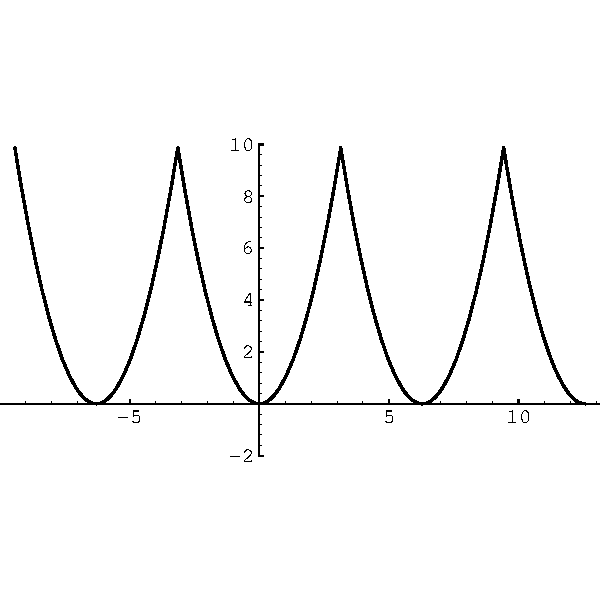
\includegraphics[width=0.6\textwidth]{ode/fourier_series/per_ext}
  \end{center}
  \caption{The periodic extension.}
  \label{per_ext_xs}
\end{figure}


\paragraph{Limited Fluctuation.}
A function that has limited total fluctuation can be written $f(x) = \psi_+(x) - \psi_-(x)$,
where $\psi_+$ and $\psi_-$ are bounded, nondecreasing functions.
An example of a function that does not have limited total fluctuation
is $\sin(1/x)$, whose fluctuation is unlimited at the point $x=0$.

\paragraph{Functions with Jump Discontinuities.}
\index{discontinuous functions}
Let $f(x)$ be a discontinuous function that has a convergent Fourier 
series.  Note that the series does not necessarily converge to $f(x)$.
Instead it converges to $\hat{f}(x) = \frac{1}{2}(f(x^-)+f(x^+))$.


\begin{Example}
  Consider the function defined by
  \[ f(x) = 
  \begin{cases}
    -x \quad &\mathrm{for}\ -\pi \leq x < 0 \\
    \pi - 2x \quad &\mathrm{for}\ 0 \leq x < \pi.
  \end{cases}
  \]
  The Fourier series converges to the function defined by
  \[ \hat{f}(x) = 
  \begin{cases}
    0 \quad &\mathrm{for}\ x = -\pi \\
    -x \quad &\mathrm{for}\ -\pi < x < 0 \\
    \pi / 2 \quad &\mathrm{for}\ x = 0 \\
    \pi - 2x \quad &\mathrm{for}\ 0 < x < \pi. 
  \end{cases}
  \]
  The function $\hat{f}(x)$ is plotted in Figure~\ref{disc_fcn}.

  \begin{figure}[h!]
    \begin{center}
      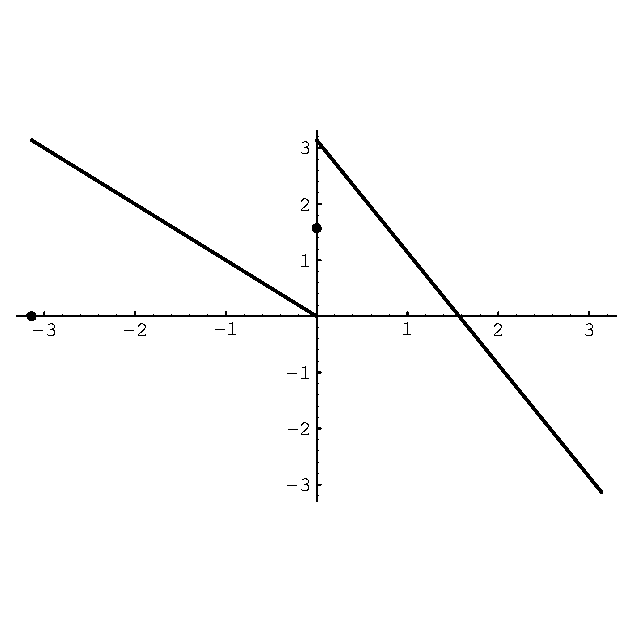
\includegraphics[width=0.6\textwidth]{ode/fourier_series/disc_fcn}
    \end{center}
    \caption{The function to which the Fourier series converges.}
    \label{disc_fcn}
  \end{figure}

\end{Example}











%%==========================================================================
\section{Least Squares Fit}
\index{least squares fit!Fourier series}



\paragraph{Approximating a function with a Fourier series.}
Suppose we want to approximate a $2\pi$-periodic function $f(x)$ with
a finite Fourier series.
\[ 
f(x) \approx \frac{a_0}{2} + \sum_{n=1}^{N} (a_n \cos(n x) + b_n \sin(n x))
\]
Here the coefficients are computed with the familiar formulas.
Is this the best approximation to the function?  That is, is it possible
to choose coefficients $\alpha_n$ and $\beta_n$ such that
\[ 
f(x) \approx \frac{\alpha_0}{2} + \sum_{n=1}^N (\alpha_n \cos(n x) + \beta_n \sin(n x)) 
\]
would give a better approximation?



\paragraph{Least squared error fit.}
The most common criterion for finding the best fit to a function is the
least squares fit.  The best approximation to a function is defined
as the one that minimizes the integral of the square of the deviation.
Thus if $f(x)$ is to be approximated on the interval $a \leq x \leq b$
by a series
\begin{equation}
  \label{eqn f = sum cn phin}
  f(x) \approx \sum_{n=1}^{N} c_n \phi_n(x),
\end{equation}
the best approximation is found by choosing values of $c_n$ that
minimize the error $E$.
\[ 
E \equiv \int_a^b \left| f(x) - \sum_{n=1}^{N} c_n \phi_n(x) \right|^2\,\dd x
\]


\paragraph{Generalized Fourier coefficients.}
We consider the case that the $\phi_n$ are orthogonal.  
For simplicity, we also assume that the $\phi_n$ are real-valued.
Then most of the terms
will vanish when we interchange the order of integration and summation.
\begin{gather*}
  E = \int_a^b \left( f^2 - 2 f \sum_{n=1}^{N} c_n \phi_n 
    + \sum_{n=1}^{N} c_n \phi_n \sum_{m=1}^{N} c_m \phi_m \right)\,\dd x
  \\
  E = \int_a^b f^2 \,\dd x - 2 \sum_{n=1}^{N} c_n \int_a^b f \phi_n \,\dd x
  + \sum_{n=1}^{N} \sum_{m=1}^{N} c_n c_m \int_a^b \phi_n \phi_m \,\dd x
  \\
  E = \int_a^b f^2 \,\dd x - 2 \sum_{n=1}^{N} c_n \int_a^b f \phi_n \,\dd x
  + \sum_{n=1}^{N} c_n^2 \int_a^b \phi_n^2 \,\dd x
  \\
  E = \int_a^b f^2 \,\dd x 
  + \sum_{n=1}^{N} \left( c_n^2 \int_a^b \phi_n^2 \,\dd x - 2 c_n \int_a^b f \phi_n \,\dd x \right)
  \\
  \intertext{We complete the square for each term.}
  E = \int_a^b f^2 \,\dd x 
  + \sum_{n=1}^{N} \left( \int_a^b \phi_n^2 \,\dd x \left( c_n 
      - \frac{ \int_a^b f \phi_n \,\dd x}{\int_a^b \phi_n^2 \,\dd x } \right)^2
    - \left( \frac{ \int_a^b f \phi_n \,\dd x}{\int_a^b \phi_n^2 \,\dd x } \right)^2 \right)
\end{gather*}
Each term involving $c_n$ is non-negative, and is minimized for
\begin{equation}
  \label{eqn cn = frac int f phi int phi2}
  c_n = \frac{ \int_a^b f \phi_n \,\dd x}{\int_a^b \phi_n^2 \,\dd x }.
\end{equation}
We call these the \textit{generalized Fourier coefficients}.

For such a choice of the $c_n$, the error is
\[
E = \int_a^b f^2 \,\dd x - \sum_{n=1}^{N} c_n^2 \int_a^b \phi_n^2 \,\dd x.
\]
Since the error is non-negative, we have
\[
\int_a^b f^2 \,\dd x \geq \sum_{n=1}^{N} c_n^2 \int_a^b \phi_n^2 \,\dd x.
\]
This is known as \textit{Bessel's Inequality}.
\index{Bessel's inequality}
If the series in Equation~\ref{eqn f = sum cn phin} converges in the mean
to $f(x)$, $\lim{N \to \infty} E = 0$, then we have equality as $N \to \infty$.
\[
\int_a^b f^2 \,\dd x = \sum_{n=1}^\infty c_n^2 \int_a^b \phi_n^2 \,\dd x.
\]
This is \textit{Parseval's equality}.
\index{Parseval's equality}




\paragraph{Fourier coefficients.}
Previously we showed that if the series,
\[ 
f(x) = \frac{a_0}{2} + \sum_{n=1}^\infty (a_n \cos(n x) + b_n \sin(n x),
\]
converges uniformly then the coefficients in the series are the Fourier 
coefficients,
\[ 
a_n = \frac{1}{\pi} \int_{-\pi}^\pi f(x) \cos(n x)\,\dd x, \qquad
b_n = \frac{1}{\pi} \int_{-\pi}^\pi f(x) \sin(n x)\,\dd x. 
\]
Now we show that by choosing the coefficients to minimize the squared error,
we obtain the same result.
We apply Equation~\ref{eqn cn = frac int f phi int phi2} to the Fourier
eigenfunctions.
\begin{gather*}
  a_0 = \frac{ \int_{-\pi}^\pi f \frac{1}{2} \,\dd x }{ \int_{-\pi}^\pi \frac{1}{4} \,\dd x }
  = \frac{1}{\pi} \int_{-\pi}^\pi f(x)\,\dd x
  \\
  a_n = \frac{ \int_{-\pi}^\pi f \cos(n x) \,\dd x }{ \int_{-\pi}^\pi \cos^2(n x) \,\dd x }
  = \frac{1}{\pi} \int_{-\pi}^\pi f(x) \cos(n x)\,\dd x
  \\
  b_n = \frac{ \int_{-\pi}^\pi f \sin(n x) \,\dd x }{ \int_{-\pi}^\pi \sin^2(n x) \,\dd x }
  = \frac{1}{\pi} \int_{-\pi}^\pi f(x) \sin(n x)\,\dd x
\end{gather*}













%%==========================================================================
\section{Fourier Series for Functions Defined on Arbitrary Ranges}






If $f(x)$ is defined on $c-d \leq x < c+d$ and $f(x + 2d) = f(x)$, then
$f(x)$ has a Fourier series of the form
\[ f(x) \sim \frac{a_0}{2} + \sum_{n=1}^\infty 
a_n \cos\left( \frac{n \pi (x+c)}{d} \right)
+ b_n \sin \left( \frac{n \pi (x+c)}{d} \right) . \]
Since
\[ \int_{c-d}^{c+d} \cos^2 \left( \frac{n \pi (x+c)}{d} \right)\,\dd x = 
\int_{c-d}^{c+d} \sin^2 \left( \frac{n \pi (x+c)}{d} \right)\,\dd x = d,\] 
the Fourier coefficients are given by the formulas
\begin{align*}
  a_n &= \frac{1}{d} \int_{c-d}^{c+d} f(x) \cos \left(
    \frac{n \pi (x+c)}{d} \right)\,\dd x \\
  b_n &= \frac{1}{d} \int_{c-d}^{c+d} f(x) \sin \left(
    \frac{n \pi (x+c)}{d} \right)\,\dd x. 
\end{align*}





\begin{Example}
  Consider the function defined by
  \[ f(x) =       \begin{cases}
    x+1 \quad &\mathrm{for}\ -1 \leq x < 0 \\
    x \quad &\mathrm{for}\ 0 \leq x < 1 \\
    3-2x \quad &\mathrm{for}\ 1 \leq x < 2.
  \end{cases}
  \]
  This function is graphed in Figure~\ref{uud12}.



  The Fourier series converges to $\hat{f}(x) = (f(x^-) + f(x^+))/2$, 
  \[ \hat{f}(x) = 
  \begin{cases}
    -\frac{1}{2} \quad &\mathrm{for}\ x = -1 \\
    x+1 \quad &\mathrm{for}\ -1 < x < 0 \\
    \frac{1}{2} \quad &\mathrm{for}\ x = 0 \\
    x \quad &\mathrm{for}\ 0 < x < 1 \\
    3-2x \quad &\mathrm{for}\ 1 \leq x < 2.
  \end{cases}
  \]
  $\hat{f}(x)$ is also graphed in Figure~\ref{uud12}.


  \begin{figure}[h!]
    \begin{center}
      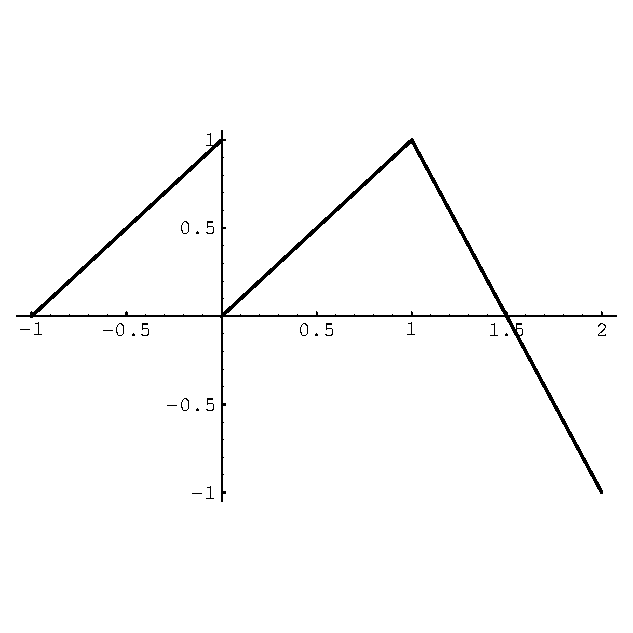
\includegraphics[width=0.49\textwidth]{ode/fourier_series/uud1}
      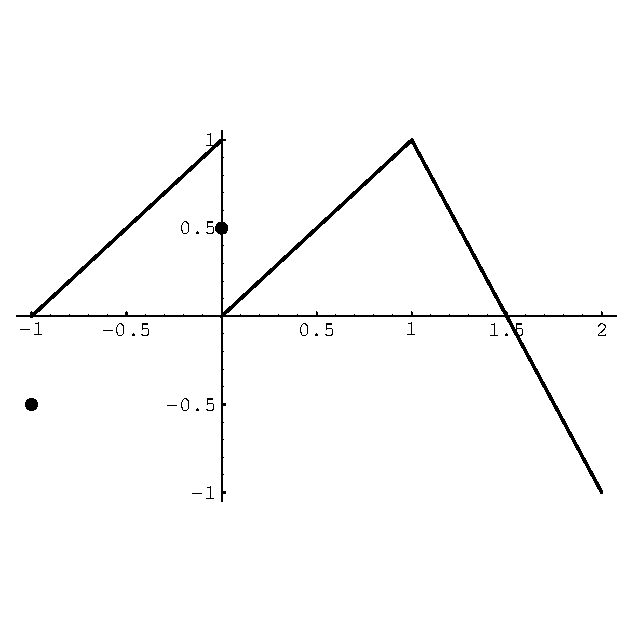
\includegraphics[width=0.49\textwidth]{ode/fourier_series/uud2}
    \end{center}
    \caption{A function defined on an interval and 
      the function to which the Fourier series converges.}
    \label{uud12}
  \end{figure}


  The Fourier coefficients are
  \begin{align*}
    a_n &= \frac{1}{3/2} \int_{-1}^2 f(x) \cos \left( \frac{2 n \pi (x+1/2)}{3}
    \right)\,\dd x \\
    &= \frac{2}{3} \int_{-1/2}^{5/2} f(x-1/2) \cos \left(
      \frac{2 n \pi x}{3} \right)\,\dd x \\
    &= \frac{2}{3} \int_{-1/2}^{1/2} (x + 1/2) \cos \left(
      \frac{2 n \pi x}{3} \right)\,\dd x 
    + \frac{2}{3} \int_{1/2}^{3/2} (x - 1/2) \cos \left(
      \frac{2 n \pi x}{3} \right)\,\dd x \\
    &\qquad \qquad+ \frac{2}{3} \int_{3/2}^{5/2} (4 - 2x) \cos \left(
      \frac{2 n \pi x}{3} \right)\,\dd x \\
    &= -\frac{1}{(n\pi)^2}\sin\left( \frac{2n\pi}{3} \right)
    \left[ 2 (-1)^n n \pi + 
      9 \sin\left(\frac{n\pi}{3}\right) \right] 
  \end{align*}
  \begin{align*}
    b_n     &= \frac{1}{3/2} \int_{-1}^2 f(x) \sin \left( \frac{2 n \pi (x+1/2)}{3}
    \right)\,\dd x \\
    &= \frac{2}{3} \int_{-1/2}^{5/2} f(x-1/2) \sin \left(
      \frac{2 n \pi x}{3} \right)\,\dd x \\
    &= \frac{2}{3} \int_{-1/2}^{1/2} (x + 1/2) \sin \left(
      \frac{2 n \pi x}{3} \right)\,\dd x 
    + \frac{2}{3} \int_{1/2}^{3/2} (x - 1/2) \sin \left(
      \frac{2 n \pi x}{3} \right)\,\dd x \\
    &\qquad \qquad + \frac{2}{3} \int_{3/2}^{5/2} (4 - 2x) \sin \left(
      \frac{2 n \pi x}{3} \right)\,\dd x \\
    &= -\frac{2}{(n\pi)^2} \sin^2\left( \frac{n\pi}{3} \right)
    \left[ 2 (-1)^n n \pi + 4 n \pi \cos\left(\frac{n\pi}{3}
      \right) - 3 \sin\left(\frac{n\pi}{3}\right) \right]
  \end{align*}


\end{Example}




%%==========================================================================
\section{Fourier Cosine Series}
\index{Fourier cosine series}

If $f(x)$ is an even function, ($f(-x) = f(x)$), then there will not be 
any sine terms in the Fourier series for $f(x)$.  The Fourier sine 
coefficient is 
\[ b_n = \frac{1}{\pi} \int_{-\pi}^\pi f(x) \sin(n x)\,\dd x.\]
Since $f(x)$ is an even function and $\sin(n x)$ is odd, $f(x) \sin(n x)$ 
is odd.  $b_n$ is the integral of an odd function from $-\pi$ to $\pi$
and is thus zero.  We can rewrite the cosine coefficients,
\begin{align*}
  a_n     &= \frac{1}{\pi} \int_{-\pi}^\pi f(x) \cos(n x)\,\dd x \\
  &= \frac{2}{\pi} \int_0^\pi f(x) \cos(n x)\,\dd x.
\end{align*}




\begin{Example}
  Consider the function defined on $[0, \pi)$ by
  \[ f(x) = 
  \begin{cases}
    x \quad &\mathrm{for}\ 0 \leq x < \pi/2 \\
    \pi - x \quad &\mathrm{for}\ \pi/2 \leq x < \pi.
  \end{cases}
  \]
  The Fourier cosine coefficients for this function are
  \begin{align*}
    a_n     &= \frac{2}{\pi} \int_0^{\pi/2} x \cos(n x)\,\dd x
    + \frac{2}{\pi} \int_{\pi/2}^\pi (\pi - x)\cos(n x)\,\dd x \\
    &=      \begin{cases}
      \frac{\pi}{4} \quad &\mathrm{for}\ n = 0, \\
      \frac{8}{\pi n^2} \cos\left(\frac{n\pi}{2}\right)
      \sin^2\left(\frac{n\pi}{4}\right)
      \quad &\mathrm{for}\ n \geq 1.
    \end{cases}
  \end{align*}
  In Figure~\ref{cos_hill_5} the even periodic extension of $f(x)$ is
  plotted in a dashed line and the sum of the first five nonzero
  terms in the Fourier cosine series are plotted in a solid line.

  \begin{figure}[h!]
    \begin{center}
      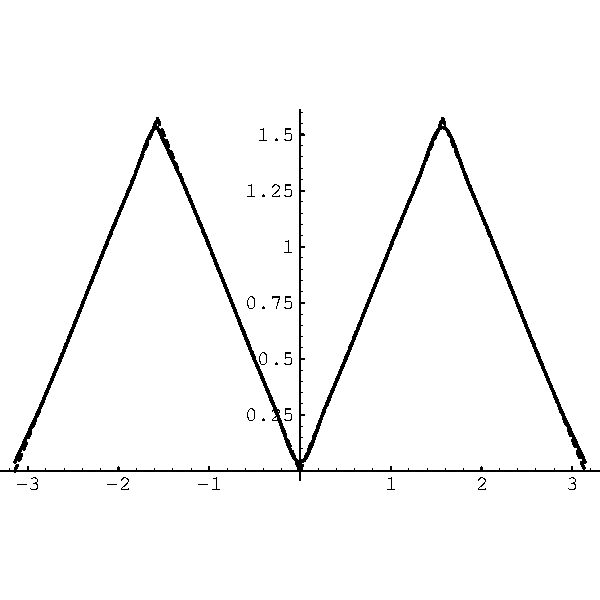
\includegraphics[width=0.6\textwidth]{ode/fourier_series/cos_h5}
    \end{center}
    \caption{Fourier Cosine series.}
    \label{cos_hill_5}
  \end{figure}
  
\end{Example}














%%==========================================================================
\section{Fourier Sine Series}
\index{Fourier Sine series}

If $f(x)$ is an odd function, ($f(-x) = - f(x)$), then there will not be any
cosine terms in the Fourier series.  Since $f(x) \cos(n x)$ is an 
odd function, the cosine coefficients will be zero.
Since $f(x) \sin(n x)$ is an even function,we can rewrite the sine coefficients
\[ b_n = \frac{2}{\pi} \int_0^\pi f(x) \sin(n x)\,\dd x.\]




\begin{Example}
  Consider the function defined on $[0, \pi)$ by
  \[ f(x) = 
  \begin{cases}
    x \quad &\mathrm{for}\ 0 \leq x < \pi/2 \\
    \pi - x \quad &\mathrm{for}\ \pi/2 \leq x < \pi.
  \end{cases}
  \]
  The Fourier sine coefficients for this function are
  \begin{align*}
    b_n     &= \frac{2}{\pi} \int_0^{\pi/2} x \sin(n x)\,\dd x
    + \frac{2}{\pi} \int_{\pi/2}^\pi (\pi - x)\sin(n x)\,\dd x \\
    &= \frac{16}{\pi n^2} \cos\left( \frac{n \pi}{4} \right)
    \sin^3\left(\frac{n \pi}{4}\right)             
  \end{align*}
  In Figure~\ref{sin_hill_5} the odd periodic extension of $f(x)$ is
  plotted in a dashed line and the sum of the first five nonzero
  terms in the Fourier sine series are plotted in a solid line.

  \begin{figure}[h!]
    \begin{center}
      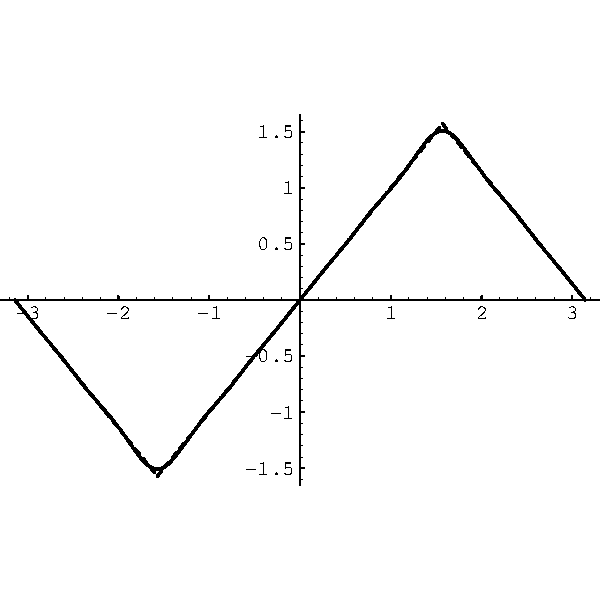
\includegraphics[width=0.6\textwidth]{ode/fourier_series/sin_h5}
    \end{center}
    \caption{Fourier Sine series.}
    \label{sin_hill_5}
  \end{figure}

\end{Example}









%%==========================================================================
\section{Complex Fourier Series and Parseval's Theorem}

By writing $\sin(n x)$ and $\cos(n x)$ in terms of $\e^{\imath n x}$ and
$\e^{-\imath n x}$ we can obtain the complex form for a Fourier series.
\begin{align*}
  \frac{a_0}{2} + \sum_{n=1}^\infty \big(a_n \cos(n x) + b_n \sin(n x)\big)
  &= \frac{a_0}{2} + \sum_{n=1}^\infty \left(a_n \frac{1}{2}(\e^{\imath n x}
    + \e^{-\imath n x}) + b_n \frac{1}{\imath 2}(\e^{\imath n x} - \e^{-\imath n x})
  \right)\\
  &= \frac{a_0}{2} + \sum_{n=1}^\infty \left(
    \frac{1}{2}(a_n - \imath b_n) \e^{\imath n x}
    + \frac{1}{2}(a_n + \imath b_n) \e^{-\imath n x} \right) \\
  &= \sum_{n=-\infty}^\infty c_n \e^{\imath n x}
\end{align*}
where
\[ c_n = 
\begin{cases}
  \frac{1}{2}(a_n - \imath b_n) \quad &\mathrm{for}\ n \geq 1 \\
  \frac{a_0}{2} \quad &\mathrm{for}\ n = 0 \\
  \frac{1}{2}(a_{-n} + \imath b_{-n}) \quad &\mathrm{for}\ n \leq -1.
\end{cases}
\]


The functions $\{ \ldots, \e^{-\imath x}, 1, \e^{\imath x}, \e^{\imath 2 x}, \ldots \}$,
satisfy the relation
\begin{align*}
  \int_{-\pi}^\pi \e^{\imath n x} \e^{-\imath m x}\,\dd x 
  &= \int_{-\pi}^\pi \e^{\imath (n-m) x}\,\dd x \\
  &= 
  \begin{cases}
    2 \pi \quad &\mathrm{for}\ n = m \\
    0 \quad &\mathrm{for}\ n \neq m.
  \end{cases}
\end{align*}

Starting with the complex form of the Fourier series of a function $f(x)$,
\[ f(x) \sim \sum_{-\infty}^\infty c_n \e^{\imath n x},\]
we multiply by $\e^{-\imath m x}$ and integrate from $-\pi$ to $\pi$ to obtain
\begin{gather*}
  \int_{-\pi}^\pi f(x) \e^{-\imath m x}\,\dd x = \int_{-\pi}^\pi 
  \sum_{-\infty}^\infty c_n \e^{\imath n x} \e^{-\imath m x}\,\dd x \\
  c_m = \frac{1}{2\pi} \int_{-\pi}^\pi f(x) \e^{-\imath m x}\,\dd x
\end{gather*}

If $f(x)$ is real-valued then
\[ c_{-m} = \frac{1}{2\pi} \int_{-\pi}^\pi f(x) \e^{\imath m x}\,\dd x
= \frac{1}{2\pi} \int_{-\pi}^\pi f(x) \overline{(\e^{-\imath m x})}\,\dd x
= \overline{c_m} \]
where $\bar{z}$ denotes the complex conjugate of $z$.

Assume that $f(x)$ has a uniformly convergent Fourier series.
\begin{align*}
  \int_{-\pi}^\pi f^2(x)\,\dd x
  &= \int_{-\pi}^\pi \left( \sum_{m = -\infty}^\infty c_m \e^{\imath m x}\right)
  \left( \sum_{n = -\infty}^\infty c_n \e^{\imath n x} \right)\,\dd x \\
  &= 2\pi \sum_{n = -\infty}^\infty c_n c_{-n} \\
  &= 2\pi \left( \sum_{n = -\infty}^{-1} \left[ \frac{1}{4}
      (a_{-n} + \imath b_{-n})(a_{-n} - \imath b_{-n}) \right]
    + \frac{a_0}{2} \frac{a_0}{2}
    + \sum_{n=1}^\infty \left[ \frac{1}{4} (a_n - \imath b_n)
      (a_n + \imath b_n) \right] \right) \\
  &= 2 \pi \left( \frac{a_0^2}{4} + \frac{1}{2} 
    \sum_{n=1}^\infty (a_n^2 + b_n^2) \right)
\end{align*}
This yields a result known as Parseval's theorem which holds even when
the Fourier series of
$f(x)$ is not uniformly convergent.



\begin{Result}
  \textbf{Parseval's Theorem. }
  If $f(x)$ has the Fourier series
  \[ f(x) \sim \frac{a_0}{2} + \sum_{n = 1}^\infty (a_n \cos(n x) + b_n \sin(n x)),\]
  then
  \[ \int_{-\pi}^\pi f^2(x)\,\dd x = \frac{\pi}{2} a_0^2
  + \pi \sum_{n = 1}^\infty (a_n^2 + b_n^2).\]
\end{Result}








%%==========================================================================
\section{Behavior of Fourier Coefficients}
\index{Fourier coefficients!behavior of}

Before we jump hip-deep into the grunge involved in determining the
behavior of the Fourier coefficients, let's take a step back and get
some perspective on what we should be looking for.  

One of the important questions is whether the Fourier series converges 
uniformly.  From Result~\ref{unif_cont} we know that a uniformly convergent
series represents a continuous function.  Thus we know that the Fourier
series of a discontinuous function cannot be uniformly convergent.
From Section~\ref{sec_unif_conv} we know that a series is uniformly
convergent if it can be bounded by a series of positive terms.  If the 
Fourier coefficients, $a_n$ and $b_n$, are $O(1/n^\alpha)$ where $\alpha>1$
then the series can be bounded by $(\mathrm{const}) \sum_{n=1}^\infty 1/n^\alpha$
and will thus be uniformly convergent. 









Let $f(x)$ be a function that meets the conditions for having a Fourier 
series and in addition is bounded.  Let $(-\pi, p_1), (p_1, p_2), (p_2, p_3),
\ldots, (p_m, \pi)$ be a partition into a finite number of intervals of the
domain, $(-\pi, \pi)$ such that on each interval $f(x)$ and all its 
derivatives are continuous.  Let $f(p^-)$ denote the left limit of $f(p)$ and 
$f(p^+)$ denote the right limit.
\[
f(p^-) = \lim_{\epsilon \to 0^+} f(p - \epsilon), \qquad
f(p^+) = \lim_{\epsilon \to 0^+} f(p + \epsilon)
\]


\begin{Example}
  The function shown in Figure~\ref{partition} would be partitioned
  into the intervals 
  \[
  (-2, -1), (-1, 0), (0, 1), (1, 2).
  \]

  \begin{figure}[h!]
    \begin{center}
      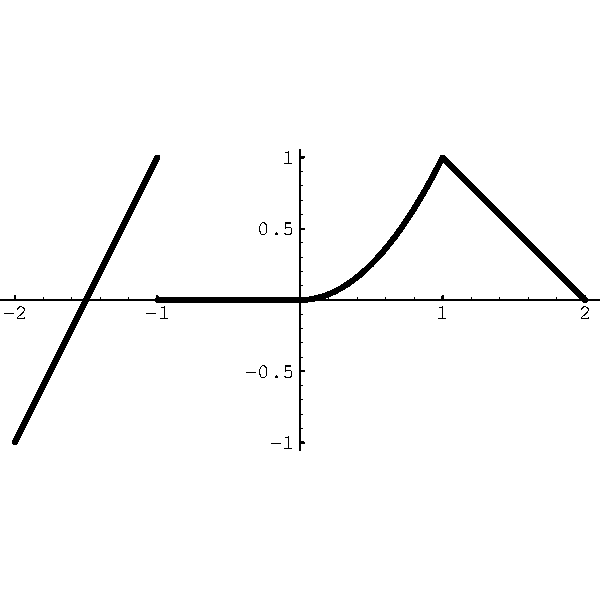
\includegraphics[width=0.6\textwidth]{ode/fourier_series/partit}
    \end{center}
    \caption{A function that can be partitioned.}
    \label{partition}
  \end{figure}

\end{Example}





Suppose $f(x)$ has the Fourier series
\[ f(x) \sim \frac{a_0}{2} + \sum_{n=1}^\infty a_n \cos(n x) + b_n \sin(n x).\]
We can use the integral formula to find the $a_n$'s.
\begin{align*}
  a_n     &= \frac{1}{\pi} \int_{-\pi}^\pi f(x) \cos(n x)\,\dd x \\
  &= \frac{1}{\pi} \left( \int_{-\pi}^{p_1} f(x) \cos(n x)\,\dd x
    + \int_{p_1}^{p_2} f(x) \cos(n x)\,\dd x + \cdots
    + \int_{p_m}^{\pi} f(x) \cos(n x)\,\dd x \right) \\
  \intertext{Using integration by parts,}
  &= \frac{1}{n\pi} \left(\Big[f(x) \sin(n x)\Big]_{-\pi}^{p_1}
    + \Big[f(x) \sin(n x)\Big]_{p_1}^{p_2} + \cdots
    + \Big[f(x) \sin(n x)\Big]_{p_m}^{\pi} \right) \\
  & \qquad \qquad - \frac{1}{n\pi} \left( \int_{-\pi}^{p_1} f'(x)\sin(n x)\,\dd x
    + \int_{p_1}^{p_2} f'(x)\sin(n x)\,\dd x
    +\int_{p_m}^{\pi} f'(x)\sin(n x)\,\dd x \right) \\
  &= \frac{1}{n\pi} \Big\{ \big[f(p_1^-)-f(p_1^+)\big]\sin(n p_1)
  + \cdots + \big[f(p_m^-)-f(p_m^+)\big]\sin(n p_m) \Big\} \\
  &\qquad \qquad - \frac{1}{n} \frac{1}{\pi} 
  \int_{-\pi}^\pi f'(x)\sin(n x)\,\dd x \\
  &= \frac{1}{n} A_n - \frac{1}{n} b_n'
\end{align*}
where 
\[ A_n = \frac{1}{\pi} \sum_{j=1}^m \sin(n p_j) 
\big[f(p_j^-) - f(p_j^+)\big] \]
and the $b_n'$ are the sine coefficients of $f'(x)$.

Since $f(x)$ is bounded, $A_n = O(1)$.  Since $f'(x)$ is bounded,
\[ b_n' = \frac{1}{\pi} \int_{-\pi}^\pi f'(x) \sin(n x)\,\dd x = O(1).\]
Thus $a_n = O(1/n)$ as $n \to \infty$.
(Actually, from the Riemann-Lebesgue Lemma, $b_n' = \mathcal{O}(1/n)$.)

Now we repeat this analysis for the sine coefficients.
\begin{align*}
  b_n     &= \frac{1}{\pi} \int_{-\pi}^\pi f(x) \sin(n x)\,\dd x \\
  &= \frac{1}{\pi} \left( \int_{-\pi}^{p_1} f(x) \sin(n x)\,\dd x
    + \int_{p_1}^{p_2} f(x) \sin(n x)\,\dd x + \cdots
    + \int_{p_m}^{\pi} f(x) \sin(n x)\,\dd x \right) \\
  &= \frac{-1}{n\pi} \Big\{\big[f(x) \cos(n x)\big]_{-\pi}^{p_1}
  + \big[f(x) \cos(n x)\big]_{p_1}^{p_2} + \cdots
  + \big[f(x) \cos(n x)\big]_{p_m}^{\pi} \Big\} \\
  & \qquad \qquad + \frac{1}{n\pi} \left( \int_{-\pi}^{p_1} f'(x)\cos(n x)\,\dd x
    + \int_{p_1}^{p_2} f'(x)\cos(n x)\,\dd x
    +\int_{p_m}^{\pi} f'(x)\cos(n x)\,\dd x \right) \\
  &= -\frac{1}{n} B_n + \frac{1}{n} a_n'
\end{align*}
where
\[ B_n = \frac{(-1)^n}{\pi} \big[f(-\pi) - f(\pi)\big] 
- \frac{1}{\pi} \sum_{j=1}^m \cos(n p_j)
\big[f(p_j^-) - f(p_j^+)\big] \]
and the $a_n'$ are the cosine coefficients of $f'(x)$.

Since $f(x)$ and $f'(x)$ are bounded, $B_n, a_n' = O(1)$ and thus
$b_n = O(1/n)$ as $n \to \infty$.

With integration by parts on the Fourier coefficients of $f'(x)$ we could
find that
\[ a_n' = \frac{1}{n} A_n' - \frac{1}{n} b_n'' \]
where $A_n' = \frac{1}{\pi} \sum_{j=1}^m \sin(n p_j)[f'(p_j^-)-f'(p_j^+)]$ and
the $b_n''$ are the sine coefficients of $f''(x)$, and
\[ b_n' = -\frac{1}{n} B_n' + \frac{1}{n} a_n'' \]
where $B_n' = \frac{(-1)^n}{\pi} [f'(-\pi) - f'(\pi)] - \frac{1}{\pi} 
\sum_{j=1}^m \cos(n p_j)
[f'(p_j^-)-f'(p_j^+)]$ and the $a_n''$ are the cosine coefficients of $f''(x)$.

Now we can rewrite $a_n$ and $b_n$ as
\begin{align*}
  a_n &= \frac{1}{n} A_n + \frac{1}{n^2} B_n' - \frac{1}{n^2} a_n'' \\
  b_n &= -\frac{1}{n} B_n + \frac{1}{n^2} A_n' - \frac{1}{n^2} b_n''.
\end{align*}

Continuing this process we could define $A_n^{(j)}$ and $B_n^{(j)}$ so that
\begin{align*}
  a_n &= \frac{1}{n} A_n + \frac{1}{n^2} B_n' - \frac{1}{n^3} A_n''
  - \frac{1}{n^4} B_n''' + \cdots \\
  b_n &= -\frac{1}{n} B_n + \frac{1}{n^2} A_n' + \frac{1}{n^3} B_n''
  - \frac{1}{n^4} A_n''' - \cdots. 
\end{align*} 




For any bounded function, the Fourier coefficients satisfy
$a_n, b_n = O(1/n)$ as $n \to \infty$.  If $A_n$ and $B_n$ are zero then the
Fourier coefficients will be $O(1/n^2)$.  A sufficient condition for this
is that the periodic extension of $f(x)$ is continuous. We see
that if the periodic extension of $f'(x)$ is continuous then $A_n'$ and 
$B_n'$ will be zero and the Fourier coefficients will be $O(1/n^3)$.


\begin{Result}
  Let $f(x)$ be a bounded function for which there is a partition of the 
  range $(-\pi, \pi)$ into a finite number of intervals such that $f(x)$ 
  and all its derivatives are continuous on each of the intervals.
  If $f(x)$ is not continuous then the Fourier coefficients are $O(1/n)$.
  If $f(x), f'(x), \ldots, f^{(k-2)}(x)$ are continuous then the Fourier
  coefficients are $O(1/n^k)$.
\end{Result}


If the periodic extension of $f(x)$ is continuous, then the Fourier 
coefficients will be $O(1/n^2)$.  The series 
$\sum_{n=1}^\infty |a_n \cos(n x) b_n \sin(n x)|$ can be bounded by
$M \sum_{n=1}^\infty 1/n^2$ where $M = { \displaystyle \max_{n} }
(|a_n| + |b_n|)$.  Thus 
the Fourier series converges to $f(x)$ uniformly.


\begin{Result}
  If the periodic extension of $f(x)$ is continuous then the Fourier
  series of $f(x)$ will converge uniformly for all $x$.
\end{Result}
\index{uniform convergence!of Fourier series}
\index{Fourier series!uniform convergence}



If the periodic extension of $f(x)$ is not continuous, we have the 
following result.

\begin{Result}
  If $f(x)$ is continuous in the interval $c < x < d$, then the Fourier
  series is uniformly convergent in the interval $c + \delta \leq x \leq
  d - \delta$ for any $\delta > 0$.
\end{Result}








\begin{Example}\textbf{Different Rates of Convergence.}

  \paragraph{A Discontinuous Function.}
  Consider the function defined by
  \[ f_1(x) = 
  \begin{cases}
    -1 \quad &\mathrm{for}\ -1 < x < 0 \\
    1, \quad &\mathrm{for}\ 0 < x < 1.
  \end{cases}
  \]
  This function has jump discontinuities, so we know that the Fourier
  coefficients are $O(1/n)$. 

  Since this function is odd, there will only be sine terms in its Fourier
  expansion.  Furthermore, since the function is symmetric about
  $x = 1/2$, there will be only odd sine terms.
  Computing these terms,
  \begin{align*}
    b_n     &= 2 \int_0^1 \sin(n \pi x)\,\dd x \\
    &= 2\left[ \frac{-1}{n\pi} \cos(n \pi x) \right]_0^1 \\
    &= 2 \left( - \frac{(-1)^n}{n \pi} - \frac{-1}{n \pi} \right) \\
    &=      \begin{cases}
      \frac{4}{n\pi} \quad &\mathrm{for odd}\ n \\
      0 \quad &\mathrm{for even}\ n.
    \end{cases}
  \end{align*}

  The function and the sum of the first three terms in the expansion
  are plotted, in dashed and solid lines respectively,
  in Figure~\ref{cont01}.  Although the three term sum
  follows the general shape of the function, it is clearly not a good
  approximation.


  \begin{figure}[h!]
    \begin{center}
      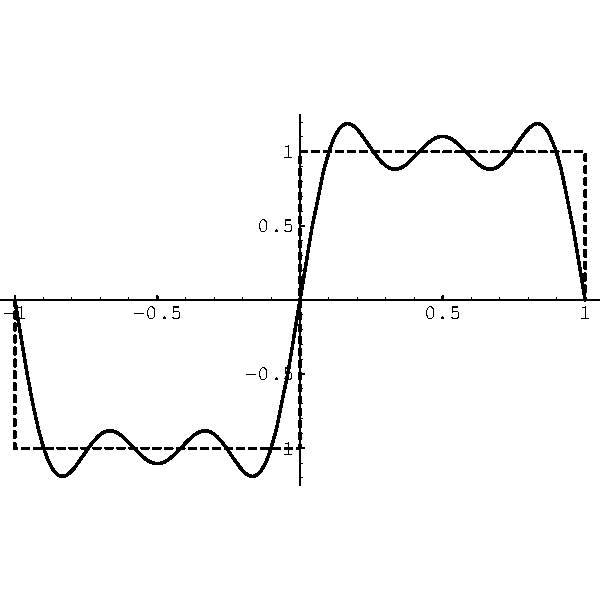
\includegraphics[width=0.49\textwidth]{ode/fourier_series/cont0}
      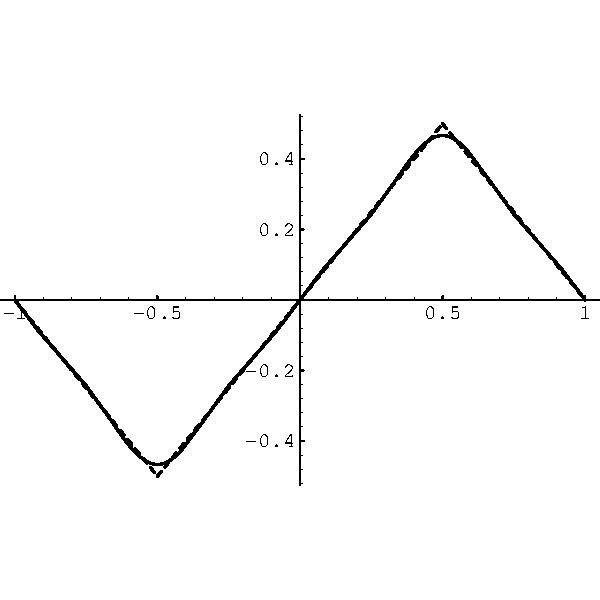
\includegraphics[width=0.49\textwidth]{ode/fourier_series/cont1}
    \end{center}
    \caption{Three term approximation for a function with 
      jump discontinuities and a continuous function.} 
    \label{cont01}
  \end{figure}


  \begin{figure}[h!]
    \begin{center}
      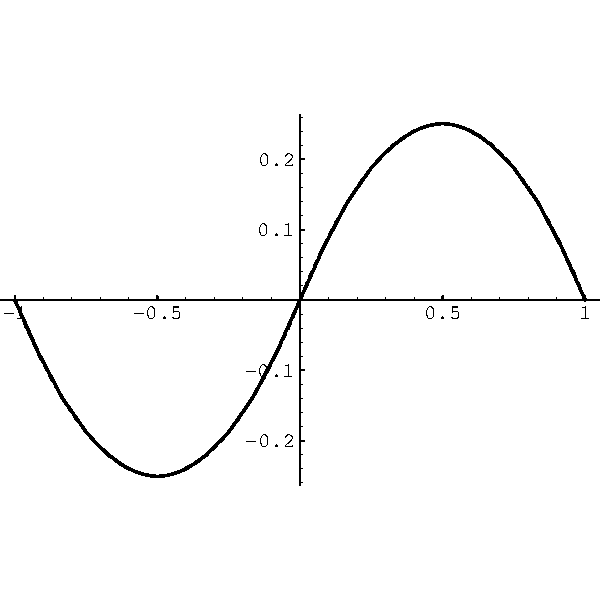
\includegraphics[width=0.49\textwidth]{ode/fourier_series/cont2}
      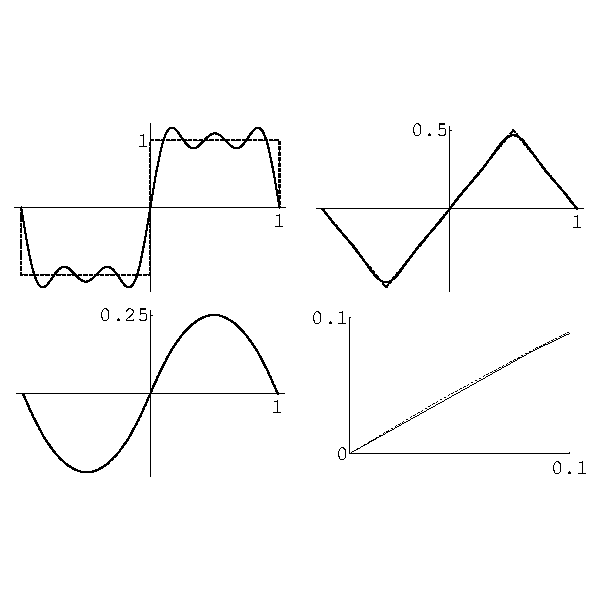
\includegraphics[width=0.49\textwidth]{ode/fourier_series/cont0124}
    \end{center}
    \caption{Three term approximation for a function with continuous
      first derivative and comparison of the rates of convergence.}
    \label{cont0124}
  \end{figure}


  \paragraph{A Continuous Function.}
  Consider the function defined by
  \[ f_2(x) = 
  \begin{cases}
    -x-1 \quad &\mathrm{for}\ -1 < x < -1/2 \\
    x \quad &\mathrm{for}\ -1/2 < x < 1/2 \\
    -x + 1 \quad &\mathrm{for}\ 1/2 < x < 1.
  \end{cases}
  \]
  Since this function is continuous, the Fourier coefficients will be $O(1/n^2)$.
  Also we see that there will only be odd sine terms in the expansion.
  \begin{align*}
    b_n     &= \int_{-1}^{-1/2} (-x-1)\sin(n\pi x)\,\dd x + 
    \int_{-1/2}^{1/2} x \sin(n\pi x)\,\dd x + 
    \int_{1/2}^1 (-x+1) \sin(n\pi x)\,\dd x \\
    &= 2\int_0^{1/2} x \sin(n \pi x)\,\dd x + 2 \int_{1/2}^1 (1-x)
    \sin(n \pi x)\,\dd x \\
    &= \frac{4}{(n\pi)^2} \sin(n\pi/2) \\
    &=      \begin{cases}
      \frac{4}{(n\pi)^2} (-1)^{(n-1)/2} \quad &\mathrm{for odd}\ n \\
      0 \quad &\mathrm{for even}\ n.
    \end{cases}
  \end{align*}

  The function and the sum of the first three terms in the expansion are plotted,
  in dashed and solid lines respectively, in Figure~\ref{cont01}.  
  We see that the convergence is much better than
  for the function with jump discontinuities.



  \paragraph{A Function with a Continuous First Derivative.}
  Consider the function defined by
  \[ f_3(x) = 
  \begin{cases}
    x(1+x) \quad &\mathrm{for}\ -1 < x < 0 \\
    x(1-x) \quad &\mathrm{for}\ 0 < x < 1.
  \end{cases}
  \]
  Since the periodic extension of this function is continuous and has a 
  continuous first derivative, the Fourier coefficients will be $O(1/n^3)$.
  We see that the Fourier expansion will contain only odd sine terms.
  \begin{align*}
    b_n     &= \int_{-1}^0 x(1+x) \sin(n \pi x)\,\dd x
    + \int_0^1 x(1-x) \sin(n \pi x)\,\dd x \\
    &= 2 \int_0^1 x(1-x) \sin(n \pi x)\,\dd x \\
    &= \frac{4(1 - (-1)^n)}{(n\pi)^3} \\
    &=      \begin{cases}
      \frac{4}{(n\pi)^3} \quad &\mathrm{for odd}\ n \\
      0 \quad &\mathrm{for even}\ n.
    \end{cases}
  \end{align*}


  The function and the sum of the first three terms in the expansion are plotted
  in Figure~\ref{cont0124}.  We see that the first three terms give a very good
  approximation to the function. The plots of the function, (in a dashed line),
  and the three term approximation, (in a solid line), are almost 
  indistinguishable.

  In Figure~\ref{cont0124} the convergence of the of the first three terms to
  $f_1(x)$, $f_2(x)$, and $f_3(x)$ are compared.  In the last graph we see a 
  closeup of $f_3(x)$ and its Fourier expansion to show the error.





\end{Example}


















%%==========================================================================
\section{Gibb's Phenomenon}
\index{Gibb's phenomenon}
The Fourier expansion of
\[ f(x) = 
\begin{cases}
  1 \quad &\mathrm{for}\ 0 \leq x < 1 \\
  -1 \quad &\mathrm{for}\ -1 \leq x < 0
\end{cases}
\]
is
\[ f(x) \sim \frac{4}{\pi} \sum_{n = 1}^\infty \frac{1}{n} \sin(n \pi x).\]
For any fixed $x$, the series converges to $\frac{1}{2}(f(x^-)+f(x^+))$.
For any $\delta > 0$, the convergence is uniform in the intervals
$-1+\delta \leq x \leq -\delta$ and $\delta \leq x \leq 1 - \delta$.
How will the nonuniform convergence at integer values of $x$
affect the Fourier series?
Finite Fourier series are plotted in Figure~\ref{gibbs} for $5$, $10$, $50$
and $100$ terms. (The plot for $100$ terms is closeup of the behavior 
near $x=0$.)  Note that at each discontinuous point there is a series of
overshoots and undershoots that are pushed closer to the discontinuity
by increasing the number of terms, but do not seem to decrease in height.
In fact, as the number of terms goes to infinity, the height of the
overshoots and undershoots does not vanish.  This is known as
Gibb's phenomenon.  


\begin{figure}[h!]
  \begin{center}
    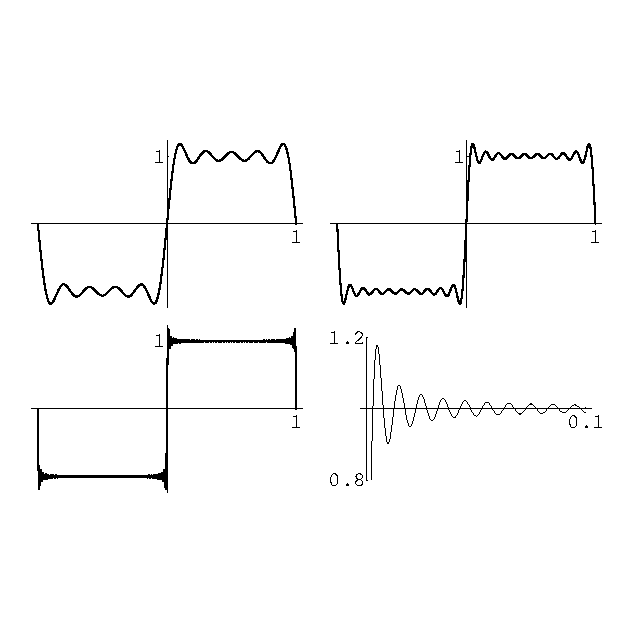
\includegraphics[width=0.6\textwidth]{ode/fourier_series/gibbs}
  \end{center}
  \caption{The finite Fourier series.}
  \label{gibbs}
\end{figure}






%%=============================================================================
\section{Integrating and Differentiating Fourier Series}

\paragraph{Integrating Fourier Series.}
Since integration is a smoothing operation, any convergent Fourier 
series can be integrated term by term to yield another convergent
Fourier series.


\begin{Example}
  Consider the step function
  \[ f(x) = 
  \begin{cases}
    \pi \quad &\mathrm{for}\ 0 \leq x < \pi \\
    -\pi \quad &\mathrm{for}\ -\pi \leq x < 0.
  \end{cases}
  \]
  Since this is an odd function, there are no cosine terms in the Fourier
  series.
  \begin{align*}
    b_n     &= \frac{2}{\pi} \int_0^\pi \pi \sin(n x)\,\dd x \\
    &= 2 \left[ -\frac{1}{n} \cos(n x) \right]_0^\pi \\
    &= \frac{2}{n} (1 - (-1)^n) \\
    &=      \begin{cases}
      \frac{4}{n} \quad &\mathrm{for odd}\ n \\
      0 \quad &\mathrm{for even}\ n.
    \end{cases}
  \end{align*}
  \[ f(x) \sim \sum_{\substack{ {n} = 1 \\ \mathrm{odd}\ n}}^{\infty} \frac{4}{n} \sin{n x} \]

  Integrating this relation,
  \begin{align*}
    \int_{-\pi}^x f(t)\,d t
    &\sim \int_{-\pi}^x \sum_{\substack{ {n} = 1 \\ \mathrm{odd}\ n}}^{\infty} \frac{4}{n} \sin(n t)\,d t \\
    F(x)    &\sim \sum_{\substack{ {n} = 1 \\ \mathrm{odd}\ n}}^{\infty} \frac{4}{n} \int_{-\pi}^x \sin(n t)\,d t \\
    &= \sum_{\substack{ {n} = 1 \\ \mathrm{odd}\ n}}^{\infty} \frac{4}{n} \left[ -\frac{1}{n} \cos(n t) 
    \right]_{-\pi}^x \\
    &= \sum_{\substack{ {n} = 1 \\ \mathrm{odd}\ n}}^{\infty}\frac{4}{n^2}(-\cos(n x) + (-1)^n) \\
    &= 4\sum_{\substack{ {n} = 1 \\ \mathrm{odd}\ n}}^{\infty} \frac{-1}{n^2} - 4 \sum_{\substack{ {n} = 1 \\ \mathrm{odd}\ n}}^{\infty} \frac{\cos(n x)}
    {n^2}
  \end{align*}
  Since this series converges uniformly,
  \[ 4\sum_{\substack{ {n} = 1 \\ \mathrm{odd}\ n}}^{\infty} \frac{-1}{n^2} - 4 \sum_{\substack{ {n} = 1 \\ \mathrm{odd}\ n}}^{\infty} \frac{\cos(n x)}{n^2}
  = F(x)
  =       \begin{cases}
    -x - \pi \quad &\mathrm{for}\ -\pi \leq x < 0 \\
    x - \pi \quad &\mathrm{for}\ 0 \leq x < \pi.
  \end{cases}
  \]
  The value of the constant term is 
  \[ 4\sum_{\substack{ {n} = 1 \\ \mathrm{odd}\ n}}^{\infty} \frac{-1}{n^2} = \frac{2}{\pi} \int_0^\pi F(x)\,\dd x
  = -\frac{1}{\pi}.\]
  Thus
  \[-\frac{1}{\pi} - 4 \sum_{\substack{ {n} = 1 \\ \mathrm{odd}\ n}}^{\infty} \frac{\cos(n x)}{n^2}
  =       \begin{cases}
    -x - \pi \quad &\mathrm{for}\ -\pi \leq x < 0 \\
    x - \pi \quad &\mathrm{for}\ 0 \leq x < \pi.
  \end{cases}
  \]

\end{Example}



\paragraph{Differentiating Fourier Series.}
Recall that in general, a series can only be differentiated if it is 
uniformly convergent.  The necessary and sufficient condition that a Fourier
series be uniformly convergent is that the periodic extension of 
the function is continuous.


\begin{Result}
  The Fourier series of a function $f(x)$ can be differentiated only if
  the periodic extension of $f(x)$ is continuous.
\end{Result}



\begin{Example}
  Consider the function defined by
  \[ f(x) =
  \begin{cases}
    \pi \quad &\mathrm{for}\ 0 \leq x < \pi \\
    -\pi \quad &\mathrm{for}\ -\pi \leq x < 0.
  \end{cases}
  \]
  $f(x)$ has the Fourier series
  \[ f(x) \sim \sum_{\substack{ {n} = 1 \\ \mathrm{odd}\ n}}^{\infty} \frac{4}{n} \sin{n x}. \]
  The function has a derivative except at the points $x = n\pi$.
  Differentiating the Fourier series yields
  \[ f'(x) \sim 4 \sum_{\substack{ {n} = 1 \\ \mathrm{odd}\ n}}^{\infty} \cos(n x).\]
  For $x \neq n\pi$, this implies
  \[ 0 = 4 \sum_{\substack{ {n} = 1 \\ \mathrm{odd}\ n}}^{\infty} \cos(n x),\]
  which is false.  The series does not converge.  This is as we expected
  since the Fourier series for $f(x)$ is not uniformly convergent.
\end{Example}







\raggedbottom
%%=============================================================================
\exercises{
\pagebreak
\flushbottom
\section{Exercises}








\begin{Exercise}
  \begin{enumerate}
  \item 
    Consider a $2 \pi$ periodic function $f(x)$ expressed as
    a Fourier series with partial sums
    \[ 
    S_N(x) = \frac{a_0}{2} + \sum_{n=1}^N a_n \cos(n x) + b_n \sin(n t). 
    \]
    Assuming that the Fourier series converges in the mean, i.e.
    \[ 
    \lim_{N \to \infty} \int_{-\pi}^\pi \left( f(x) - S_N(x) \right)^2\,\dd x = 0, 
    \]
    show 
    \[ 
    \frac{a_0^2}{2} + \sum_{n=1}^{\infty} a_n^2 +b_n^2 = \frac{1}{\pi} \int_{-\pi}^{\pi} f(x)^2 \,\dd x.
    \]
    This is called Parseval's equation. 
  \item 
    Find the Fourier series for $f(x) = x$ on $-\pi \leq x < \pi$ (and repeating
    periodically). Use this to show
    \[ 
    \sum_{n=1}^\infty \frac{1}{n^2} = \frac{\pi^2}{6}.
    \]
  \item  
    Similarly, by choosing appropriate functions $f(x)$, use 
    Parseval's equation to determine
    \[ 
    \sum_{n=1}^\infty \frac{1}{n^4} \quad \mathrm{and} \quad \sum_{n=1}^{\infty} \frac{1}{n^6}.
    \]
  \end{enumerate}
\end{Exercise}






\begin{Exercise}
  Consider the Fourier series of  $f(x) = x$ on $-\pi \leq x < \pi$ as found
  above. Investigate the convergence at the points of discontinuity.
  \begin{enumerate}
  \item 
    Let $S_N$ be the sum of the first $N$ terms in the Fourier series. Show that
    \[ 
    \frac{\dd S_N}{\dd x} = 1 - (-1)^N 
    \frac{ \cos \left( \left( N + \frac{1}{2} \right) x \right) }
    { \cos \left( \frac{x}{2} \right) }.
    \]
  \item 
    Now use this to show that 
    \[ 
    x - S_N 
    = \int_0^x \frac{ \sin \left( \left( N + \frac{1}{2} \right)(\xi - \pi) \right) }
    { \sin \left( \frac{\xi - \pi}{2} \right) }\,\dd \xi.
    \]
  \item 
    Finally investigate the maxima of this difference around $x = \pi$ and 
    provide an estimate (good to two decimal places) of the overshoot 
    in the limit $N \to \infty$.
  \end{enumerate}
\end{Exercise}








\begin{Exercise}
  Consider the boundary value problem on the interval $0 < x < 1$
  \[
  y'' + 2 y = 1 \quad y(0) = y(1) = 0.
  \]
  \begin{enumerate}
  \item 
    Choose an appropriate periodic extension and find a Fourier series solution.
  \item 
    Solve directly and find the Fourier series of the solution (using the
    same extension). Compare the result to the previous step and verify the 
    series agree.
  \end{enumerate}
\end{Exercise}






\begin{Exercise}
  Consider the boundary value problem on $0 < x < \pi$
  \[ 
  y'' + 2 y = \sin{x} \quad y'(0) = y'(\pi) = 0.
  \]
  \begin{enumerate} 
  \item 
    Find a Fourier series solution. 
  \item 
    Suppose the ODE is slightly modified: $y'' + 4 y = \sin{x}$
    with the same boundary conditions. 
    Attempt to find a Fourier series solution and discuss in as much detail as
    possible what goes wrong. 
  \end{enumerate}
\end{Exercise}








%%111111111111111111111111111111111111111111111111111111111111111111111111111111
\begin{Exercise}
  Find the Fourier cosine and sine series for $f(x) = x^2$ on $0 \leq x < \pi$.
  Are the series differentiable?
\end{Exercise}



%%222222222222222222222222222222222222222222222222222222222222222222222222222222
\begin{Exercise}
  Find the Fourier series of $\cos^n(x)$.
\end{Exercise}




%% \frac{\pi^2}{3} + 4 \sum_{n=1}^\infty \frac{(-1)^n}{n^2} \cos nx = x^2
\begin{Exercise}
  For what values of $x$ does the Fourier series
  \[
  \frac{\pi^2}{3} + 4 \sum_{n=1}^\infty \frac{(-1)^n}{n^2} \cos nx = x^2
  \]
  converge?  What is the value of the above Fourier series for all $x$? 
  From this relation show that
  \begin{gather*}
    \sum_{n = 1}^\infty \frac{1}{n^2} = \frac{\pi^2}{6} \\
    \sum_{n = 1}^\infty \frac{(-1)^{n+1}}{n^2} = \frac{\pi^2}{12}
  \end{gather*}
\end{Exercise}







%% f(x) = \cos x - 1  + \frac{2x}{\pi} ,\qquad 0 \leq x \leq \pi.
\begin{Exercise}
  \begin{enumerate}
  \item 
    Compute the Fourier sine series for the function
    \[
    f(x) = \cos x - 1  + \frac{2x}{\pi} ,\qquad 0 \leq x \leq \pi.
    \]
  \item 
    How fast do the Fourier coefficients $a_n$ where
    \[
    f(x) = \sum_{n = 1}^\infty a_n \sin n x
    \]
    decrease with increasing $n$? Explain this rate of decrease.
  \end{enumerate}
\end{Exercise}







%% Determine the cosine and sine series of f(x) = x \sin x,\qquad (0 < x < \pi)
\begin{Exercise}
  Determine the cosine and sine series of 
  \[
  f(x) = x \sin x,\qquad (0 < x < \pi).
  \]
  Estimate before doing the calculation the rate of decrease of Fourier
  coefficients, $a_n, b_n$, for large $n$.
\end{Exercise}







%% Determine the Fourier cosine series of the function f(x) = \cos \nu x
\begin{Exercise}
  Determine the Fourier cosine series of the function 
  \[
  f(x) = \cos(\nu x), \qquad 0 \leq x \leq \pi,
  \]
  where $\nu$ is an arbitrary real number. From this series deduce 
  the following identities for non-integer $\nu$.
  \begin{align*}
    \frac{\pi}{\sin(\pi \nu)} &= \frac{1}{\nu} 
    + \sum_{n = 1}^\infty (-1)^n \left( \frac{1}{\nu - n} + \frac{1}{\nu + n} \right) 
    \\
    \pi \cot(\pi \nu) &= \frac{1}{\nu}  
    + \sum_{n = 1}^\infty \left( \frac{1}{\nu - n} + \frac{1}{\nu + n} \right)
  \end{align*}
  Integrate the last formula from
  $\nu = 0$ to $\nu = \theta, (0 < \theta < 1),$ to show that
  \[
  \frac{\sin(\pi \theta)}{\pi \theta} = \prod_{n=1}^\infty \left( 1 - \frac{\theta^2}{n^2} \right).
  \]
\end{Exercise}







%% \log \cos \left( \frac{x}{2}\right) = -\log 2 - \sum_{n = 1}^\infty ...
\begin{Exercise}
  \begin{enumerate}
    %%
  \item
    Show that 
    \[
    \ln \left( \cos \left( \frac{x}{2}\right) \right) = - \ln 2 
    - \sum_{n = 1}^\infty \frac{(-1)^n}{n} \cos(n x), \qquad -\pi < x < \pi.
    \]
    Use properties of Fourier series to conclude that
    \[
    \ln \left| \cos \frac{x}{2} \right| = - \ln 2 
    - \sum_{n = 1}^\infty \frac{ (-1)^n }{ n } \cos(n x), 
    \quad x \neq (2 k + 1) \pi,\ k \in \mathbb{Z}.
    \]
    \textit{Hint: use the identity}
    \[
    \Log(1 - z) = - \sum_{n = 1}^\infty \frac{z^n}{n} \quad 
    \mathrm{for}\ |z| \leq 1, ~ z \neq 1.
    \]
    %%
  \item
    From this series deduce that 
    \[
    \int_0^\pi \ln \left( \cos \frac{x}{2} \right) \,\dd x = - \pi \ln 2.
    \]
    %%
  \item
    Show that
    \[
    \frac{1}{2} \ln \left| \frac{ \sin((x+\xi)/2) }{ \sin((x-\xi)/2) } \right|
    = \sum_{n = 1}^\infty \frac{ \sin(n x) \sin(n \xi) }{ n }, \quad
    x \neq \pm \xi + 2 k \pi.
    \]
  \end{enumerate}
\end{Exercise}









%% Eigenfunction expansion solution of ODE with homogeneous boundary conditions
\begin{Exercise}
  Solve the problem 
  \[
  y'' + \alpha y = f(x), \quad y(a) = y(b) = 0,
  \]
  with an eigenfunction expansion.  Assume that $\alpha \neq n \pi / (b-a)$,
  $n \in \mathbb{N}$.
\end{Exercise}



%% Eigenfunction expansion solution of ODE with inhomogeneous BC's
\begin{Exercise}
  Solve the problem 
  \[
  y'' + \alpha y = f(x), \quad y(a) = A, \quad y(b) = B,
  \]
  with an eigenfunction expansion.  Assume that $\alpha \neq n \pi / (b-a)$,
  $n \in \mathbb{N}$.
\end{Exercise}








%% A + \imath B \equiv \frac{1}{1-z^2} = 1 + z^2 + z^4 + \cdots \\
\begin{Exercise}
  Find the trigonometric series and the simple closed form expressions for
  $A(r,x)$ and $B(r,x)$ where $z = r \e^{\imath x}$ and 
  $|r| < 1$.
  \begin{align*}
    &\mathrm{a}) \qquad
    A + \imath B \equiv \frac{1}{1-z^2} = 1 + z^2 + z^4 + \cdots \\
    &\mathrm{b}) \qquad
    A + \imath B \equiv \log(1 + z) = z - \frac{1}{2} z^2 + \frac{1}{3} z^3 - \cdots
  \end{align*}
  Find $A_n$ and $B_n$, and the trigonometric sum for them where:
  \[
  \mathrm{c}) \qquad
  A_n + \imath B_n = 1 + z + z^2 + \cdots + z^n.
  \]
\end{Exercise}





%% \{ 1, \sin x, \cos x, \sin 2x, \cos 2x, \ldots \}
\begin{Exercise}
  \begin{enumerate}
    %%
    %%
  \item
    Is the trigonometric system
    \[
    \{ 1, \sin x, \cos x, \sin 2x, \cos 2x, \ldots \}
    \]
    orthogonal on the interval $[0,\pi]$?  Is the system orthogonal on any 
    interval of length $\pi$?  Why, in each case?
    %%
    %%
  \item
    Show that each of the systems
    \[
    \{ 1, \cos x, \cos 2x, \ldots \}, \quad \mathrm{and} \quad
    \{ \sin x, \sin 2x, \ldots \}
    \]
    are orthogonal on $[0,\pi]$.  Make them orthonormal too.
  \end{enumerate}
\end{Exercise}




%% Find $N$ such that $|f(x) - S_N(x)| < 10^{-1}$ on $|x| < \pi$.
\begin{Exercise}
  Let $S_N(x)$ be the $N^{\mathrm{th}}$ partial sum of the Fourier series for
  $f(x) \equiv |x|$ on $-\pi < x < \pi$.  Find $N$ such that 
  $|f(x) - S_N(x)| < 10^{-1}$ on $|x| < \pi$.
\end{Exercise}





%% The set $\{ \sin(n x) \}_{n=1}^\infty$ is orthogonal and complete on $[0,\pi]$.
\begin{Exercise}
  The set $\{ \sin(n x) \}_{n=1}^\infty$ is orthogonal and complete on $[0,\pi]$.
  \begin{enumerate}
    %%
    %%
  \item
    Find the Fourier sine series for $f(x) \equiv 1$ on $0 \leq x \leq \pi$.
    %%
    %%
  \item
    Find a convergent series for $g(x) = x$ on $0 \leq x \leq \pi$ by
    integrating the series for part (a).
    %%
    %%
  \item
    Apply Parseval's relation to the series in (a) to find:
    \[
    \sum_{n = 1}^\infty \frac{1}{(2n-1)^2}
    \]
    Check this result by evaluating the series in (b) at $x = \pi$.
  \end{enumerate}
\end{Exercise}





%% Show that the Fourier cosine series expansion on $[0,\pi]$ of:
\begin{Exercise}
  \begin{enumerate}
    %%
    %%
  \item
    Show that the Fourier cosine series expansion on $[0,\pi]$ of:
    \[
    f(x) \equiv
    \begin{cases}
      1,      &0 \leq x < \frac{\pi}{2}, \\
      \frac{1}{2}, &x = \frac{\pi}{2}, \\
      0,      &\frac{\pi}{2} < x \leq \pi,
    \end{cases}
    \]
    is
    \[
    S(x) = \frac{1}{2} + \frac{2}{\pi} \sum_{n = 0}^\infty \frac{ (-1)^n }{ 2n+1 }
    \cos((2n+1)x).
    \]
    %%
    %%
  \item
    Show that the $N^{\mathrm{th}}$ partial sum of the series in (a) is
    \[
    S_N(x) = \frac{1}{2} - \frac{1}{\pi} \int_0^{x - \pi/2}
    \frac{ \sin((2(N+1)t) }{ \sin t } \,d t.
    \]
    ( Hint:  Consider the difference of $\sum_{n=1}^{2N+1} (\e^{\imath y})^n$
    and $\sum_{n=1}^{N} (\e^{\imath 2 y})^n$, where $y = x - \pi/2$.)
    %%
    %%
  \item
    Show that $d S_N(x) / d x = 0$ at $x = x_n = \frac{ n \pi }{ 2(N+1) }$
    for $n = 0, 1, \ldots, N, N+2, \ldots, 2N+2$.
    %%
    %%
  \item
    Show that at $x = x_N$, the maximum of $S_N(x)$ nearest to $\pi/2$ in
    $(0,\pi/2)$ is
    \[
    S_N(x_N) = \frac{1}{2} + \frac{1}{\pi} \int_0^{\frac{ \pi N }{ 2(N+1) }}
    \frac{ \sin(2(N+1) t) }{ \sin t } \,d t.
    \]
    Clearly $x_N \uparrow \pi / 2$ as $N \to \infty$.
    %%
    %%
  \item
    Show that also in this limit,
    \[
    S_N(x_N) \to \frac{1}{2} + \frac{1}{\pi} \int_0^\pi
    \frac{ \sin t }{ t } \,d t \approx 1.0895.
    \]
    How does this compare with $f(\pi / 2 - 0)$?  This overshoot is the 
    Gibbs phenomenon that occurs at each discontinuity.  It is a manifestation
    of the non-uniform convergence of the Fourier series for $f(x)$ on
    $[0,\pi]$.
  \end{enumerate}
\end{Exercise}






%% Prove the Isoperimetric Inequality: $L^2 \geq 4 \pi A$ where $L$ is the length
\begin{Exercise}
  Prove the Isoperimetric Inequality: $L^2 \geq 4 \pi A$ where $L$ is the length
  of the perimeter and $A$ the area of any piecewise smooth plane figure.
  Show that equality is attained only for the circle.  (Hints:  The closed curve
  is represented parametrically as
  \[
  x = x(s), \quad y = y(s), \quad 0 \leq s \leq L
  \]
  where $s$ is the arclength.  In terms of $t = 2 \pi s / L$ we have
  \[
  \left( \frac{\dd x}{\dd t} \right)^2 + \left( \frac{\dd y}{\dd t} \right)^2 
  = \left( \frac{L}{2 \pi} \right)^2.
  \]
  Integrate this relation over $[0,2\pi]$.  The area is given by
  \[
  A = \int_0^{2\pi} x \frac{\dd y}{\dd t} \,d t.
  \]
  Express $x(t)$ and $y(t)$ as Fourier series and use the completeness and
  orthogonality relations to show that $L^2 - 4 \pi A \geq 0$.)
\end{Exercise}






%% g(x) = x (1-x),\ \mathrm{on}\ 0 \leq x \leq 1.
\begin{Exercise}
  \begin{enumerate}
    %%
    %%
  \item
    Find the Fourier sine series expansion and the Fourier cosine series 
    expansion of
    \[
    g(x) = x (1-x),\ \mathrm{on}\ 0 \leq x \leq 1.
    \]
    Which is better and why over the indicated interval?
    %%
    %%
  \item
    Use these expansions to show that:
    \[
    \mathrm{i)}\ 
    \sum_{k = 1}^\infty \frac{1}{k^2} = \frac{\pi^2}{6}, \quad
    \mathrm{ii)}\ 
    \sum_{k = 1}^\infty \frac{(-1)^k}{k^2} = -\frac{\pi^2}{12}, \quad
    \mathrm{iii)}\ 
    \sum_{k = 1}^\infty \frac{(-1)^k}{(2k-1)^2} = - \frac{\pi^3}{32}.
    \]
    Note: Some useful integration by parts formulas are:
    \begin{gather*}
      \int x \sin(n x) = \frac{1}{n^2} \sin(n x) - \frac{x}{n} \cos(n x); \quad
      \int x \cos(n x) = \frac{1}{n^2} \cos(n x) + \frac{x}{n} \sin(n x) \\
      \int x^2 \sin(n x) = \frac{2 x}{n^2} \sin(n x) 
      - \frac{n^2 x^2 - 2}{n^3} \cos(n x) \\
      \int x^2 \cos(n x) = \frac{2 x}{n^2} \cos(n x) 
      + \frac{n^2 x^2 - 2}{n^3} \sin(n x)
    \end{gather*}
  \end{enumerate}
\end{Exercise}








\raggedbottom
}
%%=============================================================================
\hints{
\pagebreak
\flushbottom
\section{Hints}






\begin{Hint}
  %% CONTINUE
\end{Hint}




\begin{Hint}
  %% CONTINUE
\end{Hint}




\begin{Hint}
  %% CONTINUE
\end{Hint}




\begin{Hint}
  %% CONTINUE
\end{Hint}




%%111111111111111111111111111111111111111111111111111111111111111111111111111111
\begin{Hint}
  %% CONTINUE
\end{Hint}



%%222222222222222222222222222222222222222222222222222222222222222222222222222222
\begin{Hint}
  Expand
  \[
  \cos^n(x) = \left[ \frac{1}{2} (\e^{\imath x} + \e^{-\imath x}) \right]^n
  \]
  Using Newton's binomial formula.
\end{Hint}




%% \frac{\pi^2}{3} + 4 \sum_{n=1}^\infty \frac{(-1)^n}{n^2} \cos nx = x^2
\begin{Hint}
  %% CONTINUE
\end{Hint}




%% f(x) = \cos x - 1  + \frac{2x}{\pi} ,\qquad 0 \leq x \leq \pi.
\begin{Hint}
  %% CONTINUE
\end{Hint}





%% Determine the cosine and sine series of f(x) = x \sin x,\qquad (0 < x < \pi)
\begin{Hint}
  %% CONTINUE
\end{Hint}






%% Determine the Fourier cosine series of the function f(x) = \cos \nu x
\begin{Hint}
  %% CONTINUE
\end{Hint}





%% \log \cos \left( \frac{x}{2}\right) = -\log 2 - \sum_{n = 1}^\infty ...
\begin{Hint}
  %% CONTINUE
\end{Hint}







%% Eigenfunction expansion solution of ODE with homogeneous boundary conditions
\begin{Hint}
  %% CONTINUE
\end{Hint}




%% Eigenfunction expansion solution of ODE with inhomogeneous BC's
\begin{Hint}
  %% CONTINUE
\end{Hint}





%% A + \imath B \equiv \frac{1}{1-z^2} = 1 + z^2 + z^4 + \cdots \\
\begin{Hint}
  %% CONTINUE
\end{Hint}





%% \{ 1, \sin x, \cos x, \sin 2x, \cos 2x, \ldots \}
\begin{Hint}
  %% CONTINUE
\end{Hint}





%% Find $N$ such that $|f(x) - S_N(x)| < 10^{-1}$ on $|x| < \pi$.
\begin{Hint}
  %% CONTINUE
\end{Hint}





%% The set $\{ \sin(n x) \}_{n=1}^\infty$ is orthogonal and complete on $[0,\pi]$.
\begin{Hint}
  %% CONTINUE
\end{Hint}




%% Show that the Fourier cosine series expansion on $[0,\pi]$ of:
\begin{Hint}
  %% CONTINUE
\end{Hint}





%% Prove the Isoperimetric Inequality: $L^2 \geq 4 \pi A$ where $L$ is the length
\begin{Hint}
  %% CONTINUE
\end{Hint}





%% g(x) = x (1-x),\ \mathrm{on}\ 0 \leq x \leq 1.
\begin{Hint}
  %% CONTINUE
\end{Hint}







\raggedbottom
}
%%=============================================================================
\solutions{
\pagebreak
\flushbottom
\section{Solutions}








\begin{Solution}
  \begin{enumerate}
  \item 
    We start by assuming that the Fourier series converges in the mean.
    \begin{gather*}
      \int_{-\pi}^\pi \left( f(x) - \frac{a_0}{2} 
        - \sum_{n=1}^\infty (a_n \cos(n x) + b_n \sin(n x)) \right)^2 = 0
    \end{gather*}
    We interchange the order of integration and summation.
    \begin{multline*}
      \int_{-\pi}^\pi (f(x))^2 \,\dd x  - a_0 \int_{-\pi}^\pi f(x)\,\dd x
      - 2 \sum_{n=1}^\infty \left( a_n \int_{-\pi}^\pi f(x) \cos(n x)\,\dd x 
        + b_n \int_{-\pi}^\pi f(x) \sin(n x) \right) 
      \\
      + \frac{\pi a_0^2}{2}
      + a_0 \sum_{n=1}^\infty \int_{-\pi}^\pi (a_n \cos(n x) + b_n \sin(n x))\,\dd x
      \\
      + \sum_{n=1}^\infty \sum_{m=1}^\infty \int_{-\pi}^\pi (a_n \cos(n x) + b_n \sin(n x))
      (a_m \cos(m x) + b_m \sin(m x))\,\dd x = 0
    \end{multline*}
    Most of the terms vanish because the eigenfunctions are orthogonal.
    \begin{multline*}
      \int_{-\pi}^\pi (f(x))^2 \,\dd x  - a_0 \int_{-\pi}^\pi f(x)\,\dd x
      - 2 \sum_{n=1}^\infty \left( a_n \int_{-\pi}^\pi f(x) \cos(n x)\,\dd x 
        + b_n \int_{-\pi}^\pi f(x) \sin(n x) \right) 
      \\
      + \frac{\pi a_0^2}{2}
      + \sum_{n=1}^\infty \int_{-\pi}^\pi (a_n^2 \cos^2(n x) + b_n^2 \sin^2(n x))\,\dd x = 0
    \end{multline*}
    We use the definition of the Fourier coefficients to evaluate the integrals 
    in the last sum.
    \begin{gather*}
      \int_{-\pi}^\pi (f(x))^2 \,\dd x  - \pi a_0^2
      - 2 \pi \sum_{n=1}^\infty \left( a_n^2 + b_n^2 \right) 
      + \frac{\pi a_0^2}{2}
      + \pi \sum_{n=1}^\infty \left( a_n^2 + b_n^2 \right) = 0
      \\
      \boxed{
        \frac{a_0^2}{2} + \sum_{n=1}^{\infty} \left( a_n^2 +b_n^2 \right) 
        = \frac{1}{\pi} \int_{-\pi}^{\pi} f(x)^2 \,\dd x
        }
    \end{gather*}
  \item 
    We determine the Fourier coefficients for $f(x) = x$.  Since $f(x)$ is 
    odd, all of the $a_n$ are zero.
    \begin{align*}
      b_0 &= \frac{1}{\pi} \int_{-\pi}^\pi x \sin(n x) \,\dd x
      \\
      &= \frac{1}{\pi} \left[ - \frac{1}{n} x \cos(n x) \right]_{-\pi}^\pi 
      + \int_{-\pi}^\pi \frac{1}{n} \cos(n x) \,\dd x
      \\
      &= \frac{2 (-1)^{n+1}}{n}
    \end{align*}
    The Fourier series is
    \[
    x = \sum_{n = 1}^\infty \frac{2 (-1)^{n+1}}{n} \sin(n x) \quad \mathrm{for}\ x \in (-\pi \ldots \pi).
    \]
    We apply Parseval's theorem for this series to find the value of
    $\sum_{n=1}^\infty \frac{1}{n^2}$.
    \begin{gather*}
      \sum_{n = 1}^\infty \frac{4}{n^2} = \frac{1}{\pi} \int_{-\pi}^\pi x^2 \,\dd x
      \\
      \sum_{n = 1}^\infty \frac{4}{n^2} = \frac{2 \pi^2}{3}
      \\
      \boxed{
        \sum_{n=1}^\infty \frac{1}{n^2} = \frac{\pi^2}{6}
        }
    \end{gather*}
  \item  
    Consider $f(x) = x^2$.
    Since the function is even, there are no sine terms in the Fourier series.
    The coefficients in the cosine series are
    \begin{align*}
      a_0 &= \frac{2}{\pi} \int_0^\pi x^2\,\dd x 
      \\
      &= \frac{2 \pi^2}{3} 
      \\
      a_n &= \frac{2}{\pi} \int_0^\pi x^2 \cos(n x)\,\dd x 
      \\
      &= \frac{4(-1)^n}{n^2}.
    \end{align*}
    Thus the Fourier series is
    \[ 
    x^2 = \frac{\pi^2}{3} + 4 \sum_{n=1}^\infty \frac{(-1)^n}{n^2} \cos(n x)
    \quad \mathrm{for}\ x \in (-\pi \ldots \pi).
    \]
    We apply Parseval's theorem for this series to find the value of
    $\sum_{n=1}^\infty \frac{1}{n^4}$.
    \begin{gather*}
      \frac{2 \pi^4}{9} + 16 \sum_{n = 1}^\infty \frac{1}{n^4} = \frac{1}{\pi} \int_{-\pi}^\pi x^4 \,\dd x
      \\
      \frac{2 \pi^4}{9} + 16 \sum_{n = 1}^\infty \frac{1}{n^4} = \frac{2 \pi^4}{5}
      \\
      \boxed{
        \sum_{n=1}^\infty \frac{1}{n^4} = \frac{\pi^4}{90}
        }
    \end{gather*}
    Now we integrate the series for $f(x) = x^2$.
    \begin{gather*}
      \int_0^x \left( \xi^2 - \frac{\pi^2}{3} \right)\,\dd \xi 
      = 4 \sum_{n=1}^\infty \frac{(-1)^n}{n^2} \int_0^x \cos(n \xi)\,\dd \xi
      \\
      \frac{x^3}{3} - \frac{\pi^2}{3} x = 4 \sum_{n=1}^\infty \frac{(-1)^n}{n^3} \sin(n x)
    \end{gather*}
    We apply Parseval's theorem for this series to find the value of
    $\sum_{n=1}^\infty \frac{1}{n^6}$.
    \begin{gather*}
      16 \sum_{n = 1}^\infty \frac{1}{n^6} 
      = \frac{1}{\pi} \int_{-\pi}^\pi \left( \frac{x^3}{3} - \frac{\pi^2}{3} x \right)^2 \,\dd x
      \\
      16 \sum_{n = 1}^\infty \frac{1}{n^6} = \frac{16 \pi^6}{945}
      \\
      \boxed{
        \sum_{n=1}^\infty \frac{1}{n^6} = \frac{\pi^6}{945}
        }
    \end{gather*}
  \end{enumerate}
\end{Solution}









\begin{Solution}
  \begin{enumerate}
  \item 
    We differentiate the partial sum of the Fourier series and evaluate the sum.
    \begin{gather*}
      S_N = \sum_{n = 1}^N \frac{2 (-1)^{n+1}}{n} \sin(n x)
      \\
      S_N' = 2 \sum_{n = 1}^N (-1)^{n+1} \cos(n x)
      \\
      S_N' = 2 \Re \left( \sum_{n = 1}^N (-1)^{n+1} \e^{\imath n x} \right)
      \\
      S_N' = 2 \Re \left( \frac{ 1 - (-1)^{N+2} \e^{\imath (N + 1) x} }{ 1 + \e^{\imath x} } \right)
      \\
      S_N' = \Re \left( \frac{ 1 + \e^{-\imath x} - (-1)^N \e^{\imath (N + 1) x} 
          - (-1)^N \e^{\imath N x} }{ 1 + \cos(x) } \right)
      \\
      S_N' = 1 - (-1)^N \frac{ \cos((N + 1) x) + \cos(N x) }
      { 1 + \cos(x) }
      \\
      S_N' = 1 - (-1)^N \frac{ \cos \left( \left( N + \frac{1}{2} \right) x \right)
        \cos \left( \frac{x}{2} \right) }
      { \cos^2 \left( \frac{x}{2} \right) }
      \\
      \boxed{
        \frac{\dd S_N}{\dd x} = 1 - (-1)^N 
        \frac{ \cos \left( \left( N + \frac{1}{2} \right) x \right) }
        { \cos \left( \frac{x}{2} \right) }
        }
    \end{gather*}
  \item 
    We integrate $S_N'$.
    \begin{gather*}
      S_N(x) - S_N(0) = x 
      - \int_0^x \frac{ (-1)^N \cos \left( \left( N + \frac{1}{2} \right) \xi \right) }
      { \cos \left( \frac{\xi}{2} \right) } \,\dd \xi
      \\
      \boxed{
        x - S_N 
        = \int_0^x \frac{ \sin \left( \left( N + \frac{1}{2} \right)(\xi - \pi) \right) }
        { \sin \left( \frac{\xi - \pi}{2} \right) }\,\dd \xi
        }
    \end{gather*}
  \item 
    We find the extrema of the overshoot $E = x - S_N$ with the first 
    derivative test.
    \[
    E' = \frac{ \sin \left( \left( N + \frac{1}{2} \right)(x - \pi) \right) }
    { \sin \left( \frac{x - \pi}{2} \right) } = 0
    \]
    We look for extrema in the range $(-\pi \ldots \pi)$.
    \begin{gather*}
      \left( N + \frac{1}{2} \right)(x - \pi) = - n \pi
      \\
      x = \pi \left( 1 - \frac{n}{N + 1/2} \right), \quad n \in [1 \ldots 2 N]
    \end{gather*}
    The closest of these extrema to $x = \pi$ is
    \[
    x = \pi \left( 1 - \frac{1}{N + 1/2} \right)
    \]
    Let $E_0$ be the overshoot at this point.
    We approximate $E_0$ for large $N$.
    \begin{gather*}
      E_0 = \int_0^{\pi(1-1/(N+1/2))} 
      \frac{ \sin \left( \left( N + \frac{1}{2} \right)(\xi - \pi) \right) }
      { \sin \left( \frac{\xi - \pi}{2} \right) }\,\dd \xi
      \\
      \intertext{We shift the limits of integration.}
      E_0 = \int_{\pi/(N+1/2)}^\pi
      \frac{ \sin \left( \left( N + \frac{1}{2} \right)\xi \right) }
      { \sin \left( \frac{\xi}{2} \right) }\,\dd \xi
      \\
      \intertext{We add and subtract an integral over $[0 \ldots \pi/(N+1/2)]$.}
      E_0 = \int_0^\pi \frac{ \sin \left( \left( N + \frac{1}{2} \right)\xi \right) }
      { \sin \left( \frac{\xi}{2} \right) }\,\dd \xi
      - \int_0^{\pi/(N+1/2)}
      \frac{ \sin \left( \left( N + \frac{1}{2} \right)\xi \right) }
      { \sin \left( \frac{\xi}{2} \right) }\,\dd \xi
    \end{gather*}
    We can evaluate the first integral with contour integration on the unit
    circle $C$.
    \begin{align*}
      \int_0^\pi \frac{ \sin \left( \left( N + \frac{1}{2} \right)\xi \right) }
      { \sin \left( \frac{\xi}{2} \right) }\,\dd \xi
      &= \int_0^\pi \frac{ \sin \left( \left( 2 N + 1 \right) \xi \right) }
      { \sin \left( \xi \right) }\,\dd \xi
      \\
      &= \frac{1}{2} \int_{-\pi}^\pi \frac{ \sin \left( \left( 2 N + 1 \right) \xi \right) }
      { \sin \left( \xi \right) }\,\dd \xi
      \\
      &= \frac{1}{2} \pv \int_C \frac{ \Im \left( z^{2 N + 1} \right) }{(z - 1/z)/(\imath 2)}
      \frac{\dd z}{\imath z}
      \\
      &= \Im \left( \pv \int_C \frac{ z^{2 N + 1} }{(z^2 - 1)} \,\dd z \right)
      \\
      &= \Im \left( \imath \pi \Res \left( \frac{ z^{2 N + 1} }{(z + 1)(z - 1)}, 1 \right)
        + \imath \pi \Res \left( \frac{ z^{2 N + 1} }{(z + 1)(z - 1)}, - 1 \right) \right)
      \\
      &= \pi \Re \left( \frac{ 1^{2 N + 1} }{ 2 }
        + \frac{ (-1)^{2 N + 1} }{ -2 } \right)
      \\
      &= \pi 
    \end{align*}
    We approximate the second integral.
    \begin{align*}
      \int_0^{\pi/(N+1/2)}
      \frac{ \sin \left( \left( N + \frac{1}{2} \right)\xi \right) }
      { \sin \left( \frac{\xi}{2} \right) }\,\dd \xi
      &= \frac{2}{2 N + 1}
      \int_0^\pi \frac{ \sin(x) }{ \sin \left( \frac{x}{2 N + 1} \right) }\,\dd x
      \\
      &\approx 2 \int_0^\pi \frac{ \sin(x) }{ x }\,\dd x
      \\
      &= 2 \int_0^\pi \frac{ 1 }{ x } \sum_{n = 0}^\infty \frac{(-1)^n x^{2 n + 1}}{ (2 n + 1)! } \,\dd x
      \\
      &= 2 \sum_{n = 0}^\infty \int_0^\pi \frac{(-1)^n x^{2 n}}{ (2 n + 1)! } \,\dd x
      \\
      &= 2 \sum_{n = 0}^\infty \frac{(-1)^n \pi^{2 n + 1}}{ (2 n + 1) (2 n + 1)! } \,\dd x
      \\
      &\approx 3.70387
    \end{align*}
    In the limit as $N \to \infty$, the overshoot is 
    \[
    | \pi - 3.70387| \approx 0.56.
    \]
  \end{enumerate}
\end{Solution}












\begin{Solution}
  \begin{enumerate}
  \item 
    The eigenfunctions of the self-adjoint problem
    \[
    -y'' = \lambda y, \quad y(0) = y(1) = 0,
    \]
    are 
    \[
    \phi_n = \sin(n \pi x), \quad n \in \mathbb{Z}^+
    \]
    We find the series expansion of the inhomogeneity $f(x) = 1$.
    \begin{gather*}
      1 = \sum_{n = 1}^\infty f_n \sin(n \pi x)
      \\
      f_n = 2 \int_0^1 \sin(n \pi x) \,\dd x 
      \\
      f_n = 2 \left[ - \frac{ \cos(n \pi x) }{ n \pi } \right]_0^1
      \\
      f_n = \frac{2}{n \pi} (1 - (-1)^n)
      \\
      f_n = \begin{cases}
        \frac{4}{n \pi} &\mathrm{for odd}\ n \\
        0 &\mathrm{for even}\ n
      \end{cases}
    \end{gather*}
    We expand the solution in a series of the eigenfunctions.
    \[
    y = \sum_{n = 1}^\infty a_n \sin(n \pi x)
    \]
    We substitute the series into the differential equation.
    \begin{gather*}
      y'' + 2 y = 1
      \\
      - \sum_{n = 1}^\infty a_n \pi^2 n^2 \sin(n \pi x) + 2 \sum_{n = 1}^\infty a_n \sin(n \pi x)
      = \sum_{\substack{n = 1 \\ \mathrm{odd}\ n}}^\infty \frac{4}{n \pi} \sin(n \pi x)
      \\
      a_n = \begin{cases}
        \frac{4}{n \pi (2 - \pi^2 n^2)} &\mathrm{for odd}\ n \\
        0 &\mathrm{for even}\ n
      \end{cases}
      \\
      \boxed{
        y = \sum_{\substack{n = 1 \\ \mathrm{odd}\ n}}^\infty \frac{4}{n \pi (2 - \pi^2 n^2)} \sin(n \pi x)
        }
    \end{gather*}
  \item 
    Now we solve the boundary value problem directly.  
    \[
    y'' + 2 y = 1 \quad y(0) = y(1) = 0
    \]
    The general solution of the differential equation is
    \[
    y = c_1 \cos \left( \sqrt{2} x \right) + c_2 \sin \left( \sqrt{2} x \right)
    + \frac{1}{2}.
    \]
    We apply the boundary conditions to find the solution.
    \begin{gather*}
      c_1 + \frac{1}{2} = 0, \quad  
      c_1 \cos \left( \sqrt{2} \right) 
      + c_2 \sin \left( \sqrt{2} \right) + \frac{1}{2} = 0
      \\
      c_1 = - \frac{1}{2}, \quad
      c_2 = \frac{ \cos \left( \sqrt{2} \right) - 1 }
      { 2 \sin \left( \sqrt{2} \right) }
      \\
      \boxed{
        y = \frac{1}{2} \left( 1 - \cos \left( \sqrt{2} x \right) 
          +  \frac{ \cos \left( \sqrt{2} \right) - 1 }
          { \sin \left( \sqrt{2} \right) } \sin \left( \sqrt{2} x \right) \right)
        }
    \end{gather*}
    We find the Fourier sine series of the solution.
    \begin{gather*}
      y = \sum_{n = 1}^\infty a_n \sin(n \pi x)
      \\
      a_n = 2 \int_0^1 y(x) \sin(n \pi x) \,\dd x 
      \\
      a_n = \int_0^1  \left( 1 - \cos \left( \sqrt{2} x \right) 
        +  \frac{ \cos \left( \sqrt{2} \right) - 1 }
        { \sin \left( \sqrt{2} \right) } \sin \left( \sqrt{2} x \right) \right)
      \sin(n \pi x) \,\dd x 
      \\
      a_n = \frac{2 (1 - (-1)^2}{n \pi (2 - \pi^2 n^2)}
      \\
      a_n = \begin{cases}
        \frac{4}{n \pi (2 - \pi^2 n^2)} &\mathrm{for odd}\ n \\
        0 &\mathrm{for even}\ n
      \end{cases}
    \end{gather*}
    We obtain the same series as in the first part.
  \end{enumerate}
\end{Solution}







\begin{Solution}
  \begin{enumerate} 
  \item 
    The eigenfunctions of the self-adjoint problem
    \[
    -y'' = \lambda y, \quad y'(0) = y'(\pi) = 0,
    \]
    are 
    \[
    \phi_0 = \frac{1}{2}, \quad \phi_n = \cos(n x), \quad n \in \mathbb{Z}^+
    \]
    We find the series expansion of the inhomogeneity $f(x) = \sin(x)$.
    \begin{gather*}
      f(x) = \frac{f_0}{2} + \sum_{n = 1}^\infty f_n \cos(n x)
      \\
      f_0 = \frac{2}{\pi} \int_0^\pi \sin(x) \,\dd x 
      \\
      f_0 = \frac{4}{\pi}
      \\
      f_n = \frac{2}{\pi} \int_0^\pi \sin(x) \cos(n x)\,\dd x 
      \\
      f_n = \frac{ 2 (1 + (-1)^n) }{ \pi (1 - n^2) }
      \\
      f_n = \begin{cases}
        \frac{ 4 }{ \pi (1 - n^2) } &\mathrm{for even}\ n \\
        0 &\mathrm{for odd}\ n
      \end{cases}
    \end{gather*}
    We expand the solution in a series of the eigenfunctions.
    \[
    y = \frac{a_0}{2} + \sum_{n = 1}^\infty a_n \cos(n x)
    \]
    We substitute the series into the differential equation.
    \begin{gather*}
      y'' + 2 y = \sin(x)
      \\
      - \sum_{n = 1}^\infty a_n n^2 \cos(n x) + a_0 + 2 \sum_{n = 1}^\infty a_n \cos(n x)
      = \frac{2}{\pi} 
      + \sum_{\substack{n = 2 \\ \mathrm{even}\ n}}^\infty \frac{ 4 }{ \pi (1 - n^2) } \cos(n x)
      \\
      \boxed{
        y = \frac{1}{\pi}
        + \sum_{\substack{n = 2 \\ \mathrm{even}\ n}}^\infty \frac{ 4 }{ \pi (1 - n^2)(2 - n^2) } \cos(n x)
        }
    \end{gather*}
  \item 
    We expand the solution in a series of the eigenfunctions.
    \[
    y = \frac{a_0}{2} + \sum_{n = 1}^\infty a_n \cos(n x)
    \]
    We substitute the series into the differential equation.
    \begin{gather*}
      y'' + 4 y = \sin(x)
      \\
      - \sum_{n = 1}^\infty a_n n^2 \cos(n x) + 2 a_0 + 4 \sum_{n = 1}^\infty a_n \cos(n x)
      = \frac{2}{\pi} 
      + \sum_{\substack{n = 2 \\ \mathrm{even}\ n}}^\infty \frac{ 4 }{ \pi (1 - n^2) } \cos(n x)
    \end{gather*}
    It is not possible to solve for the $a_2$ coefficient.  That equation is
    \[
    (0) a_2 = - \frac{4}{3 \pi}.
    \]
    This problem is to be expected, as this boundary value problem does not 
    have a solution.
    The solution of the differential equation is
    \[
    y  = c_1 \cos(2 x) + c_2 \sin(2 x) + \frac{1}{3} \sin(x)
    \]
    The boundary conditions give us an inconsistent set of constraints.
    \begin{gather*}
      y'(0) = 0, \quad y'(\pi) = 0
      \\
      c_2 + \frac{1}{3} = 0, \quad c_2 - \frac{1}{3} = 0
    \end{gather*}
    Thus the problem has no solution.
  \end{enumerate}
\end{Solution}









%%111111111111111111111111111111111111111111111111111111111111111111111111111111
\begin{Solution}

  \textbf{Cosine Series.}
  The coefficients in the cosine series are
  \begin{align*}
    a_0     &= \frac{2}{\pi} \int_0^\pi x^2\,\dd x \\
    &= \frac{2 \pi^2}{3} \\
    a_n     &= \frac{2}{\pi} \int_0^\pi x^2 \cos(n x)\,\dd x \\
    &= \frac{4(-1)^n}{n^2}.
  \end{align*}
  Thus the Fourier cosine series is
  \[ f(x) = \frac{\pi^2}{3} + \sum_{n = 1}^\infty \frac{4(-1)^n}{n^2} \cos(n x).\]
  In Figure~\ref{cos_sin_xs} the even periodic extension of $f(x)$ is plotted
  in a dashed line and the sum of the first five terms in the Fourier
  series is plotted in a solid line.
  Since the even periodic extension is continuous, the cosine series is
  differentiable.

  \begin{figure}[h!]
    \begin{center}
      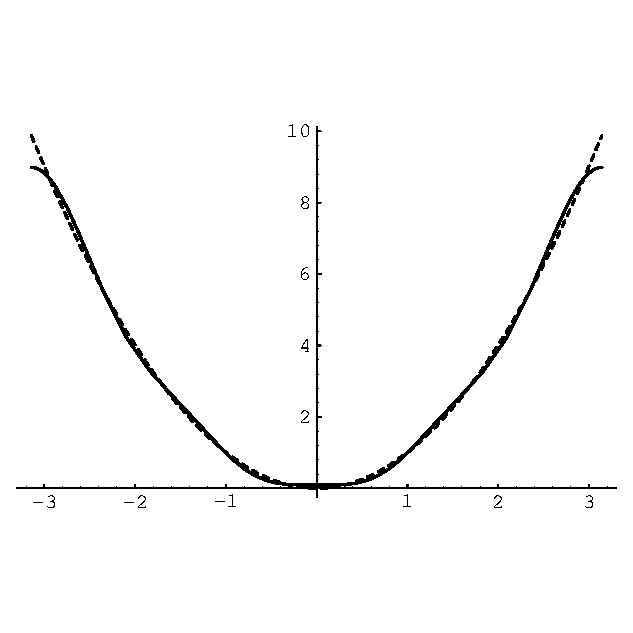
\includegraphics[width=0.49\textwidth]{ode/fourier_series/cos_xs}
      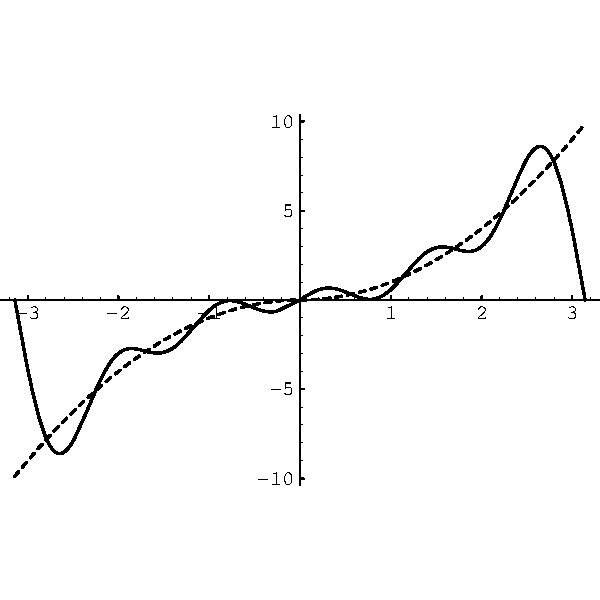
\includegraphics[width=0.49\textwidth]{ode/fourier_series/sin_xs}
    \end{center}
    \caption{The Fourier cosine and sine series.}
    \label{cos_sin_xs}
  \end{figure}


  \textbf{Sine Series.}
  The coefficients in the sine series are
  \begin{align*}
    b_n     &= \frac{2}{\pi} \int_0^\pi x^2 \sin(n x)\,\dd x \\
    &= -\frac{2(-1)^n \pi}{n} - \frac{4(1 - (-1)^n)}{\pi n^3} \\
    &=      \begin{cases}
      -\frac{2(-1)^n \pi}{n} \quad &\mathrm{for even}\ n \\
      -\frac{2(-1)^n \pi}{n} - \frac{8}{\pi n^3} \quad 
      &\mathrm{for odd}\ n.
    \end{cases}
  \end{align*}
  Thus the Fourier sine series is
  \[ f(x) \sim - \sum_{n = 1}^\infty \left(\frac{2(-1)^n \pi}{n} 
    + \frac{4(1 - (-1)^n)}{\pi n^3} \right) \sin(n x).\]
  In Figure~\ref{cos_sin_xs} the odd periodic extension of $f(x)$ and the sum
  of the first five terms in the sine series are plotted.
  Since the odd periodic extension of $f(x)$ is not continuous, the series
  is not differentiable.
\end{Solution}











%%222222222222222222222222222222222222222222222222222222222222222222222222222222
\begin{Solution}
  We could find the expansion by integrating to find the Fourier
  coefficients, but it is easier to expand $\cos^n(x)$ directly.
  \begin{align*}
    \cos^n(x)
    &= \left[ \frac{1}{2} (\e^{\imath x} + \e^{-\imath x}) \right]^n \\
    &= \frac{1}{2^n} \left[ \binom{n}{0} \e^{\imath n x} +
      \binom{n}{1} \e^{\imath (n-2)x} + \cdots +
      \binom{n}{n-1} \e^{-\imath (n-2)x} + \binom{n}{n} \e^{-\imath n x} \right]
  \end{align*}
  If $n$ is odd,
  \begin{align*}
    \cos^n(x)
    &= \frac{1}{2^n} \Bigg[ \binom{n}{0} (\e^{\imath n x} + \e^{-\imath n x})
    + \binom{n}{1} (\e^{\imath (n-2)x} + \e^{-\imath (n-2)x}) + \cdots \\
    &\qquad\qquad + \binom{n}{(n-1)/2}(\e^{\imath x} + \e^{-\imath x}) \Bigg] \\
    &= \frac{1}{2^n} \left[ \binom{n}{0} 2 \cos(n x)
      + \binom{n}{1} 2 \cos((n-2)x) + \cdots +
      \binom{n}{(n-1)/2}2\cos(x) \right] \\
    &= \frac{1}{2^{n-1}} \sum_{m=0}^{(n-1)/2} \binom{n}{m}
    \cos((n-2m)x) \\
    &= \frac{1}{2^{n-1}} \sum_{\substack{k = 1 \\ \mathrm{odd}\ k}}^n
    \binom{ n }{ (n-k)/2 } \cos(k x).
  \end{align*}
  If $n$ is even,
  \begin{align*}
    \cos^n(x)
    &= \frac{1}{2^n} \Bigg[ \binom{n}{0}(\e^{\imath n x}+\e^{-\imath n x})
    + \binom{n}{1} (\e^{\imath (n-2)x}+\e^{-\imath (n-2)x}) + \cdots \\
    &\qquad\qquad + \binom{n}{n/2-1} (\e^{\imath 2 x}+\e^{-i2x}) 
    + \binom{n}{n/2}\Bigg] \\
    &= \frac{1}{2^n} \left[ \binom{n}{0}2\cos(n x)
      + \binom{n}{1} 2\cos((n-2)x) + \cdots +
      \binom{n}{n/2-1} 2\cos(2x) + \binom{n}{n/2}\right] \\
    &= \frac{1}{2^n} \binom{n}{n/2} + \frac{1}{2^{n-1}} \sum_{m=0}^{(n-2)/2}
    \binom{n}{m} \cos((n-2m)x) \\
    &= \frac{1}{2^n} \binom{n}{n/2} 
    + \frac{1}{2^{n-1}} \sum_{\substack{k = 2 \\ \mathrm{even}\ k}}^n
    \binom{ n }{ (n-k)/2 } \cos(k x).
  \end{align*}
  We may denote,
  \[
  \boxed{
    \cos^n(x) = \frac{a_0}{2} \sum_{k = 1}^n a_k \cos(k x),
    }
  \]
  where
  \[
  \boxed{
    a_k = \frac{ 1 + (-1)^{n-k} }{2} \frac{1}{2^{n-1}} \binom{ n }{ (n-k)/2 }.
    }
  \]
\end{Solution}




%% \frac{\pi^2}{3} + 4 \sum_{n=1}^\infty \frac{(-1)^n}{n^2} \cos nx = x^2
\begin{Solution}
  We expand $f(x)$ in a cosine series. The coefficients in the cosine series are
  \begin{align*}
    a_0     &= \frac{2}{\pi} \int_0^\pi x^2\,\dd x \\
    &= \frac{2 \pi^2}{3} \\
    a_n     &= \frac{2}{\pi} \int_0^\pi x^2 \cos(n x)\,\dd x \\
    &= \frac{4(-1)^n}{n^2}.
  \end{align*}
  Thus the Fourier cosine series is
  \[ 
  f(x) = \frac{\pi^2}{3} + 4 \sum_{n = 1}^\infty \frac{(-1)^n}{n^2} \cos(n x).
  \]
  The Fourier series converges to the even periodic extension of 
  \[
  f(x) = x^2 \quad \mathrm{for}\ 0 < x < \pi,
  \]
  which is 
  \[
  \boxed{
    \hat{f}(x) = \left( x - 2 \pi \left( \left\lfloor \frac{x + \pi}{2\pi} 
        \right\rfloor \right) \right)^2.
    }
  \]
  ($\lfloor \cdot \rfloor$ denotes the floor or greatest integer function.)
  This periodic extension is a continuous function.  Since $x^2$ is an 
  even function, we have
  \[
  \boxed{
    \frac{\pi^2}{3} + 4 \sum_{n=1}^\infty \frac{(-1)^n}{n^2} \cos nx = x^2
    \quad \mathrm{for}\ -\pi \leq x \leq \pi.
    }
  \]

  We substitute $x = \pi$ into the Fourier series.
  \begin{gather*}
    \frac{\pi^2}{3} + 4 \sum_{n=1}^\infty \frac{(-1)^n}{n^2} \cos(n\pi) = \pi^2 \\
    \boxed{
      \sum_{n = 1}^\infty \frac{1}{n^2} = \frac{\pi^2}{6}
      }
  \end{gather*}

  We substitute $x = 0$ into the Fourier series.
  \begin{gather*}
    \frac{\pi^2}{3} + 4 \sum_{n=1}^\infty \frac{(-1)^n}{n^2} = 0 \\
    \boxed{
      \sum_{n = 1}^\infty \frac{(-1)^{n+1}}{n^2} = \frac{\pi^2}{12}
      }
  \end{gather*}
\end{Solution}




%% f(x) = \cos x - 1  + \frac{2x}{\pi} ,\qquad 0 \leq x \leq \pi.
\begin{Solution}
  \begin{enumerate}
    %%
    %%
  \item 
    We compute the Fourier sine coefficients.
    \begin{align*}
      a_n 
      &= \frac{2}{\pi} \int_0^\pi f(x) \sin(n x) \,\dd x \\
      &= \frac{2}{\pi} \int_0^\pi 
      \left( \cos x - 1 + \frac{2 x}{\pi} \right) \sin(n x) \,\dd x \\
      &= \frac{2 (1 + (-1)^n)}{\pi (n^3 - n)}
    \end{align*}
    \[
    \boxed{
      a_n = 
      \begin{cases}
        \frac{4}{\pi (n^3 - n)} &\mathrm{for even}\ n \\
        0 &\mathrm{for odd}\ n
      \end{cases}
      }
    \]
    %%
    %%
  \item 
    From our work in the previous part, we see that the Fourier coefficients
    decay as $1/n^3$. The Fourier sine series converges to the odd periodic 
    extension of the function, $\hat{f}(x)$.  We can determine the rate 
    of decay of the Fourier
    coefficients from the smoothness of $\hat{f}(x)$.
    For $-\pi < x < \pi$, the odd periodic extension of $f(x)$ is defined
    \[
    \hat{f}(x) = \begin{cases}
      f(x) = \cos(x) - 1 + \frac{2 x}{\pi} &0 \leq x < \pi, \\
      -f(-x) = - \cos(x) + 1 + \frac{2 x}{\pi} &-\pi \leq x < 0.
    \end{cases}
    \]
    Since 
    \[
    \hat{f}(0^+) = \hat{f}(0^-) = 0 
    \quad \mathrm{and} \quad
    \hat{f}(\pi) = \hat{f}(-\pi) = 0
    \]
    $\hat{f}(x)$ is continuous, $C^0$.  Since
    \[
    \hat{f}'(0^+) = \hat{f}'(0^-) = \frac{2}{\pi} 
    \quad \mathrm{and} \quad
    \hat{f}'(\pi) = \hat{f}'(- \pi) = \frac{2}{\pi}
    \]
    $\hat{f}(x)$ is continuously differentiable, $C^1$.  However, since
    \[
    \hat{f}''(0^+) = -1, 
    \quad \mathrm{and} \quad
    \hat{f}''(0^-) = 1
    \]
    $\hat{f}(x)$ is not $C^2$.
    Since $\hat{f}(x)$ is $C^1$ we know that the Fourier coefficients decay
    as $1 / n^3$.
  \end{enumerate}
\end{Solution}





%% Determine the cosine and sine series of f(x) = x \sin x,\qquad (0 < x < \pi)
\begin{Solution}
  \textbf{Cosine Series.}
  The even periodic extension of $f(x)$ is a $C^0$, continuous, function
  (See Figure~\ref{xsinx_cos_ser}.
  Thus the coefficients in the cosine series will decay as $1/n^2$.
  The Fourier cosine coefficients are
  \begin{align*}
    a_0     &= \frac{2}{\pi} \int_0^\pi x \sin x \,\dd x \\
    &= 2
  \end{align*}
  \begin{align*}
    a_1     &= \frac{2}{\pi} \int_0^\pi x \sin x \cos x \,\dd x \\
    &= - \frac{1}{2}
  \end{align*}
  \begin{align*}
    a_n     &= \frac{2}{\pi} \int_0^\pi x \sin x \cos(n x) \,\dd x \\
    &= \frac{2 (-1)^{n+1}}{n^2-1}, \quad \mathrm{for}\ n \geq 2
  \end{align*}
  The Fourier cosine series is
  \[
  \boxed{
    \hat{f}(x) = 1 - \frac{1}{2} \cos x 
    -2 \sum_{n=2}^\infty \frac{2 (-1)^n}{n^2-1} \cos(n x).
    }
  \]
  \begin{figure}[h!]
    \begin{center}
      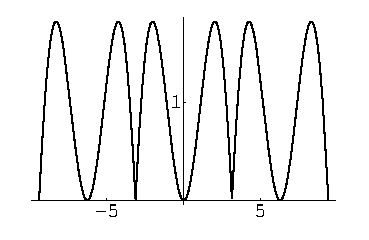
\includegraphics[width=0.4\textwidth]{ode/fourier_series/xsinx_cos_ser}
    \end{center}
    \caption{The even periodic extension.}
    \label{xsinx_cos_ser}
  \end{figure}




  \textbf{Sine Series.}
  The odd periodic extension of $f(x)$ is a $C^1$, continuously differentiable,
  function (See Figure~\ref{xsinx_sin_ser}.
  Thus the coefficients in the cosine series will decay as $1/n^3$.
  The Fourier sine coefficients are
  \begin{align*}
    a_1     &= \frac{1}{\pi} \int_0^\pi x \sin x \sin x \,\dd x \\
    &= \frac{\pi}{2}
  \end{align*}
  \begin{align*}
    a_n     &= \frac{2}{\pi} \int_0^\pi x \sin x \sin(n x) \,\dd x \\
    &= - \frac{4 (1 + (-1)^n) n}{\pi(n^2-1)^2}, \quad \mathrm{for}\ n \geq 2
  \end{align*}
  The Fourier sine series is
  \[
  \boxed{
    \hat{f}(x) = \frac{\pi}{2} \sin x 
    - \frac{4}{\pi} \sum_{n=2}^\infty \frac{(1 + (-1)^n)n}{(n^2-1)^2} 
    \cos(n x).
    }
  \]
  \begin{figure}[h!]
    \begin{center}
      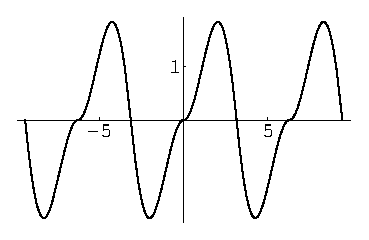
\includegraphics[width=0.4\textwidth]{ode/fourier_series/xsinx_sin_ser}
    \end{center}
    \caption{The odd periodic extension.}
    \label{xsinx_sin_ser}
  \end{figure}
\end{Solution}






%% Determine the Fourier cosine series of the function f(x) = \cos \nu x
\begin{Solution}
  If $\nu = n$ is an integer, then the Fourier cosine series is the single term 
  $\cos(|n| x)$.  We assume that $\nu \neq n$.

  We note that the even periodic extension of 
  $\cos(\nu x)$ is $C^0$ so that the series converges to $\cos(\nu x)$ for
  $-\pi \leq x \leq \pi$ and the coefficients decay as $1/n^2$.
  We compute the Fourier cosine coefficients.
  \begin{align*}
    a_0 &= \frac{2}{\pi} \int_0^\pi \cos(\nu x) \,\dd x 
    \\
    &= \frac{2 \sin(\pi \nu)}{\pi \nu} 
  \end{align*}
  \begin{align*}
    a_n &= \frac{2}{\pi} \int_0^\pi \cos(\nu x) \cos(n x)\,\dd x 
    \\
    &= (-1)^n \left( \frac{1}{\nu - n} + \frac{1}{\nu + n} \right) 
    \sin(\pi \nu)
  \end{align*}
  The Fourier cosine series is
  \[
  \boxed{
    \cos(\nu x) = \frac{\sin(\pi \nu)}{\pi \nu} 
    + \sum_{n = 1}^\infty (-1)^n \left( \frac{1}{\nu - n} + \frac{1}{\nu + n} \right) 
    \sin(\pi \nu) \cos(n x).
    }
  \]

  We substitute $x = 0$ into the Fourier cosine series.
  \begin{gather*}
    1 = \frac{\sin(\pi \nu)}{\pi \nu} 
    + \sum_{n = 1}^\infty (-1)^n \left( \frac{1}{\nu - n} + \frac{1}{\nu + n} \right) \sin(\pi \nu)
    \\
    \boxed{
      \frac{\pi}{\sin \pi \nu} = \frac{1}{\nu} 
      + \sum_{n = 1}^\infty (-1)^n \left( \frac{1}{\nu - n} + \frac{1}{\nu + n} \right)
      }
  \end{gather*}

  Next we substitute $x = \pi$ into the Fourier cosine series.
  \begin{gather*}
    \cos(\nu \pi) = \frac{\sin(\pi \nu)}{\pi \nu} 
    + \sum_{n = 1}^\infty (-1)^n \left( \frac{1}{\nu - n} + \frac{1}{\nu + n} \right) 
    \sin(\pi \nu) (-1)^n 
    \\
    \boxed{
      \pi \cot \pi \nu = \frac{1}{\nu}  
      + \sum_{n = 1}^\infty \left( \frac{1}{\nu - n } + \frac{1}{\nu + n} \right)
      }
  \end{gather*}

  Note that neither $\cot(\pi \nu)$ nor $1 / \nu$ is integrable at $\nu = 0$.
  We write the last formula so each side is integrable.
  \[
  \pi \cot \pi \nu - \frac{1}{\nu} 
  = \sum_{n = 1}^\infty \left( \frac{1}{\nu - n } + \frac{1}{\nu + n} \right)
  \]
  We integrate from $\nu = 0$ to $\nu = \theta < 1$.
  \begin{gather*}
    \left[ \ln \left( \frac{\sin(\pi \nu)}{\nu} \right) \right]_0^\theta
    = \sum_{n = 1}^\infty \left( \left[ \ln(n - \nu) \right]_0^\theta
      + \left[ \ln(n + \nu) \right]_0^\theta \right) 
    \\
    \ln \left( \frac{\sin(\pi \theta)}{\theta} \right) - \ln \pi
    = \sum_{n = 1}^\infty \left( \ln \left( \frac{n - \theta}{n} \right)
      + \ln \left( \frac{n + \theta}{n} \right) \right) 
    \\
    \ln \left( \frac{\sin(\pi \theta)}{\pi \theta} \right)
    = \sum_{n = 1}^\infty \ln \left( 1 - \frac{\theta^2}{n^2} \right) 
    \\
    \ln \left( \frac{\sin(\pi \theta)}{\pi \theta} \right)
    = \ln \left( \prod_{n=1}^\infty \left( 1 - \frac{\theta^2}{n^2} \right) \right) 
    \\
    \boxed{
      \frac{\sin(\pi \theta)}{\pi \theta} = \prod_{n=1}^\infty \left( 1 - \frac{\theta^2}{n^2} \right)
      }
  \end{gather*}
\end{Solution}





%% \log \cos \left( \frac{x}{2}\right) = -\log 2 - \sum_{n = 1}^\infty ...
\begin{Solution}
  \begin{enumerate}
    %%
    %%
  \item
    We will consider the principal branch of the logarithm, 
    $-\pi < \Im(\Log z) \leq \pi$.  For $-\pi < x < \pi$, $\cos(x/2)$ is 
    positive so that $\ln(\cos(x/2))$ is well-defined.  At $x = \pm \pi$,
    $\ln(\cos(x/2))$ is singular.  However, the function is integrable so
    it has a Fourier series which converges except at $x = (2 k + 1) \pi$, 
    $k \in \mathbb{Z}$.
    \begin{align*}
      \ln \left( \cos \frac{x}{2} \right)
      &= \ln \left( \frac{ \e^{\imath x / 2} + \e^{-\imath x / 2} }{ 2 } \right) 
      \\
      &= - \ln 2 + \ln \left( \e^{-\imath x / 2} \left( 1 + \e^{\imath x} \right)
      \right) 
      \\
      &= - \ln 2 - \imath \frac{x}{2} + \Log \left( 1 + \e^{\imath x} \right) 
      \\
      \intertext{Since $|\e^{\imath x}| \leq 1$ and $\e^{\imath x} \neq -1$ for 
        $\Im(x) \geq 0$, $x \neq (2 k + 1) \pi$, 
        we can expand the last term in a Taylor series in that domain.}
      &= - \ln 2 - \imath \frac{x}{2} - \sum_{n = 1}^\infty \frac{ (-1)^n }{ n } 
      \left( \e^{\imath x} \right)^n 
      \\
      &= - \ln 2 - \sum_{n = 1}^\infty \frac{ (-1)^n }{ n } \cos(n x)
      - \imath \left( \frac{x}{2} + \sum_{n = 1}^\infty \frac{ (-1)^n }{ n } \sin(n x) \right) 
    \end{align*}
    For $-\pi < x < \pi$, $\ln(\cos(x/2))$ is real-valued.
    We equate the real parts of the equation on this domain to obtain the 
    desired Fourier series.
    \[
    \boxed{
      \ln \left( \cos \left( \frac{x}{2} \right) \right) = - \ln 2 
      - \sum_{n = 1}^\infty \frac{ (-1)^n }{ n } \cos(n x), \quad -\pi < x < \pi.
      }
    \]
    The domain of convergence for this series is $\Im(x) = 0$, $x \neq (2 k + 1) \pi$.
    The Fourier series converges to the periodic extension of the function.
    \[
    \boxed{
      \ln \left| \cos \frac{x}{2} \right| = - \ln 2 
      - \sum_{n = 1}^\infty \frac{ (-1)^n }{ n } \cos(n x), 
      \quad x \neq (2 k + 1) \pi,\ k \in \mathbb{Z}
      }
    \]
    %%
    %%
  \item
    Now we integrate the function from $0$ to $\pi$.
    \begin{align*}
      \int_0^\pi \ln \left( \cos \frac{x}{2} \right) \,\dd x
      &= \int_0^\pi \left( - \ln 2 
        - \sum_{n = 1}^\infty \frac{ (-1)^n }{ n } \cos(n x) \right) \,\dd x 
      \\
      &= - \pi \ln 2 
      - \sum_{n = 1}^\infty \frac{ (-1)^n }{ n } \int_0^\pi \cos(n x)\,\dd x 
      \\
      &= - \pi \ln 2 - \sum_{n = 1}^\infty \frac{ (-1)^n }{ n } 
      \left[ \frac{\sin(n x)}{n} \right]_0^\pi 
    \end{align*}
    \[
    \boxed{
      \int_0^\pi \ln \left( \cos \left( \frac{x}{2} \right) \right) \,\dd x 
      = - \pi \ln 2
      }
    \]
    %%
    %%
  \item
    We expand the logorithm.
    \[
    \frac{1}{2} \ln \left| \frac{ \sin((x+\xi)/2) }{ \sin((x-\xi)/2) } \right|
    = \frac{1}{2} \ln \left| \sin((x+\xi)/2) \right| 
    - \frac{1}{2} \ln \left| \sin((x-\xi)/2) \right| 
    \]
    Consider the function $\ln |\sin(y/2)|$.  Since 
    $\sin(x) = \cos(x - \pi / 2)$, we can use the result of part (a) to obtain,
    \begin{align*}
      \ln \left| \sin \left( \frac{y}{2} \right) \right|
      &= \ln \left| \cos \left( \frac{y - \pi}{2} \right) \right| 
      \\
      &= - \ln 2 - \sum_{n = 1}^\infty \frac{ (-1)^n }{ n } \cos( n (y - \pi) ) 
      \\
      &= - \ln 2 - \sum_{n = 1}^\infty \frac{ 1 }{ n } \cos( n y ), \quad
      \mathrm{for}\ y \neq 2 \pi k,\ k \in \mathbb{Z}.
    \end{align*}
    We return to the original function:
    \[
    \frac{1}{2} \ln \left| \frac{ \sin((x+\xi)/2) }{ \sin((x-\xi)/2) } \right|
    = \frac{1}{2} \left( 
      - \ln 2 - \sum_{n = 1}^\infty \frac{ 1 }{ n } \cos( n (x + \xi) )
      + \ln 2 + \sum_{n = 1}^\infty \frac{ 1 }{ n } \cos( n (x - \xi) ) \right), 
    \]
    for $x \pm \xi \neq 2 \pi k$, $k \in \mathbb{Z}$.
    \[
    \boxed{
      \frac{1}{2} \ln \left| \frac{ \sin((x+\xi)/2) }{ \sin((x-\xi)/2) } \right|
      = \sum_{n = 1}^\infty \frac{ \sin(n x) \sin(n \xi) }{ n }, \quad
      x \neq \pm \xi + 2 k \pi
      }
    \]
  \end{enumerate}
\end{Solution}







%% Eigenfunction expansion solution of ODE with homogeneous boundary conditions
\begin{Solution}
  The eigenfunction problem associated with this problem is
  \[
  \phi'' + \lambda^2 \phi = 0, \quad \phi(a) = \phi(b) = 0,
  \]
  which has the solutions,
  \[
  \lambda_n = \frac{n \pi}{b-a}, \quad
  \phi_n = \sin \left( \frac{ n \pi (x-a) }{ b-a } \right), \quad
  n \in \mathbb{N}.
  \]
  We expand the solution and the inhomogeneity in the eigenfunctions.
  \[
  y(x) = \sum_{n = 1}^\infty y_n \sin \left( \frac{ n \pi (x-a) }{ b-a } \right)
  \]
  \[
  f(x) = \sum_{n = 1}^\infty f_n \sin \left( \frac{ n \pi (x-a) }{ b-a } \right), \quad
  f_n = \frac{2}{b-a} \int_a^b f(x) \sin \left( \frac{ n \pi (x-a) }{ b-a }
  \right) \,\dd x
  \]
  Since the solution $y(x)$ satisfies the same homogeneous boundary conditions
  as the eigenfunctions, we can differentiate the series.  We substitute
  the series expansions into the differential equation.
  \begin{gather*}
    y'' + \alpha y = f(x) \\
    \sum_{n = 1}^\infty y_n \left( -\lambda_n^2 + \alpha \right)
    \sin \left( \lambda_n x \right)
    = \sum_{n = 1}^\infty f_n \sin \left( \lambda_n x \right) \\
    y_n = \frac{ f_n }{ \alpha - \lambda_n^2 }
  \end{gather*}
  Thus the solution of the problem has the series representation,
  \[
  \boxed{
    y(x) = \sum_{n = 1}^\infty \left( \alpha - \lambda_n^2 \right)
    \sin \left( \frac{ n \pi (x-a) }{ b-a } \right).
    }
  \]
\end{Solution}



%% Eigenfunction expansion solution of ODE with inhomogeneous BC's
\begin{Solution}
  The eigenfunction problem associated with this problem is
  \[
  \phi'' + \lambda^2 \phi = 0, \quad \phi(a) = \phi(b) = 0,
  \]
  which has the solutions,
  \[
  \lambda_n = \frac{n \pi}{b-a}, \quad
  \phi_n = \sin \left( \frac{ n \pi (x-a) }{ b-a } \right), \quad
  n \in \mathbb{N}.
  \]
  We expand the solution and the inhomogeneity in the eigenfunctions.
  \[
  y(x) = \sum_{n = 1}^\infty y_n \sin \left( \frac{ n \pi (x-a) }{ b-a } \right)
  \]
  \[
  f(x) = \sum_{n = 1}^\infty f_n \sin \left( \frac{ n \pi (x-a) }{ b-a } \right), \quad
  f_n = \frac{2}{b-a} \int_a^b f(x) \sin \left( \frac{ n \pi (x-a) }{ b-a }
  \right) \,\dd x
  \]
  Since the solution $y(x)$ does not satisfy the same homogeneous boundary 
  conditions as the eigenfunctions, we can differentiate the series.  
  We multiply the differential equation by an eigenfunction and integrate
  from $a$ to $b$.  We use integration by parts to move derivatives 
  from $y$ to the eigenfunction.
  \begin{gather*}
    y'' + \alpha y = f(x) \\
    \int_a^b y''(x) \sin( \lambda_m x)\,\dd x 
    + \alpha \int_a^b y(x) \sin( \lambda_m x)\,\dd x 
    = \int_a^b f(x) \sin( \lambda_m x)\,\dd x \\
    \left[ y' \sin( \lambda_m x) \right]_a^b
    - \int_a^b y' \lambda_m \cos( \lambda_m x)\,\dd x 
    + \alpha \frac{b-a}{2} y_m
    = \frac{b-a}{2} f_m \\
    - \left[ y \lambda_m \cos( \lambda_m x ) \right]_a^b
    - \int_a^b y \lambda_m^2 \sin( \lambda_m x)\,\dd x 
    + \alpha \frac{b-a}{2} y_m
    = \frac{b-a}{2} f_m \\
    - B \lambda_m (-1)^m + A \lambda_m (-1)^{m+1}
    - \lambda_m^2 y_m
    + \alpha \frac{b-a}{2} y_m
    = \frac{b-a}{2} f_m \\
    y_m = \frac{ f_m + (-1)^m \lambda_m (A+B) }{\alpha - \lambda_m^2} 
  \end{gather*}
  Thus the solution of the problem has the series representation,
  \[
  \boxed{
    y(x) = \sum_{n = 1}^\infty 
    \frac{ f_m + (-1)^m \lambda_m (A+B) }{\alpha - \lambda_m^2} 
    \sin \left( \frac{ n \pi (x-a) }{ b-a } \right).
    }
  \]
\end{Solution}










%% A + \imath B \equiv \frac{1}{1-z^2} = 1 + z^2 + z^4 + \cdots \\
\begin{Solution}
  \begin{enumerate}
    %%
    %%
  \item
    \begin{align*}
      A + \imath B
      &= \frac{1}{1-z^2} \\
      &= \sum_{n = 0}^\infty z^{2n} \\
      &= \sum_{n = 0}^\infty r^{2n} \e^{\imath 2 n x} \\
      &= \sum_{n = 0}^\infty r^{2n} \cos(2 n x) + \imath \sum_{n = 1}^\infty r^{2n} \sin(2 n x)
    \end{align*}
    \[
    \boxed{
      A = \sum_{n = 0}^\infty r^{2n} \cos(2 n x), \qquad
      B = \sum_{n = 1}^\infty r^{2n} \sin(2 n x)
      }
    \]
    \begin{align*}
      A + \imath B
      &= \frac{1}{1-z^2} \\
      &= \frac{1}{ 1 - r^2 \e^{\imath 2 x} } \\
      &= \frac{1}{ 1 - r^2 \cos(2 x) - \imath r^2 \sin(2 x) } \\
      &= \frac{1 - r^2 \cos(2 x) + \imath r^2 \sin(2 x) }
      { ( 1 - r^2 \cos(2 x) )^2 + ( r^2 \sin (2 x) )^2 }
    \end{align*}
    \[
    \boxed{
      A = \frac{1 - r^2 \cos(2 x) }{ 1 - 2 r^2 \cos(2 x) + r^4 }, \qquad
      B = \frac{ r^2 \sin(2 x) }{ 1 - 2 r^2 \cos(2 x) + r^4 }
      }
    \]
    %%
    %%
  \item
    We consider the principal branch of the logarithm.
    \begin{align*}
      A + \imath B
      &= \log(1 + z) \\
      &= \sum_{n = 1}^\infty \frac{ (-1)^{n+1} }{ n } z^n \\
      &= \sum_{n = 1}^\infty \frac{ (-1)^{n+1} }{ n } r^n \e^{\imath n x} \\
      &= \sum_{n = 1}^\infty \frac{ (-1)^{n+1} }{ n } r^n 
      \big( \cos(n x) + \imath \sin(n x) \big)
    \end{align*}
    \[
    \boxed{
      A = \sum_{n = 1}^\infty \frac{ (-1)^{n+1} }{ n } r^n \cos(n x), \qquad
      B = \sum_{n = 1}^\infty \frac{ (-1)^{n+1} }{ n } r^n \sin(n x)
      }
    \]
    \begin{align*}
      A + \imath B
      &= \log(1 + z) \\
      &= \log \left(1 + r \e^{\imath x} \right) \\
      &= \log \left(1 + r \cos x + \imath r \sin x \right) \\
      &= \log \left| 1 + r \cos x + \imath r \sin x \right| 
      + \imath \arg \left( 1 + r \cos x + \imath r \sin x \right) \\
      &= \log \sqrt{ ( 1 + r \cos x )^2 + ( r \sin x )^2 } 
      + \imath \arctan \left( 1 + r \cos x, r \sin x \right) 
    \end{align*}
    \[
    \boxed{
      A = \frac{1}{2} \log \left( 1 + 2 r \cos x + r^2 \right), \qquad
      B = \arctan \left( 1 + r \cos x, r \sin x \right) 
      }
    \]
    %%
    %%
  \item
    \begin{align*}
      A_n + \imath B_n
      &= \sum_{k=1}^n z^k \\
      &= \frac{1 - z^{n+1}}{1-z} \\
      &= \frac{ 1 - r^{n+1} \e^{\imath (n+1) x} }{ 1 - r \e^{\imath x} } \\
      &= \frac{ 1 - r \e^{- \imath x} - r^{n+1} \e^{\imath (n+1) x} 
        + r^{n+2} \e^{\imath n x} }{ 1 - 2 r \cos x + r^2 }
    \end{align*}
    \[
    \boxed{
      A_n = \frac{ 1 - r \cos x - r^{n+1} \cos((n+1)x) + r^{n+2} \cos(n x) }
      { 1 - 2 r \cos x + r^2 }
      }
    \]
    \[
    \boxed{
      B_n = \frac{ r \sin x - r^{n+1} \sin((n+1)x) + r^{n+2} \sin(n x) }
      { 1 - 2 r \cos x + r^2 }
      }
    \]
    \begin{align*}
      A_n + \imath B_n
      &= \sum_{k=1}^n z^k \\
      &= \sum_{k=1}^n r^k \e^{\imath k x}
    \end{align*}
    \[
    \boxed{
      A_n = \sum_{k=1}^n r^k \cos(k x), \qquad
      B_n = \sum_{k=1}^n r^k \sin(k x)
      }
    \]
  \end{enumerate}
\end{Solution}





%% \{ 1, \sin x, \cos x, \sin 2x, \cos 2x, \ldots \}
\begin{Solution}
  \begin{enumerate}
    %%
    %%
  \item
    \[
    \int_0^\pi 1 \cdot \sin x \,\dd x = \left[ - \cos x \right]_0^\pi = 2
    \]
    Thus the system is not orthogonal on the interval $[0,\pi]$.  Consider the
    interval $[a,a+\pi]$.
    \begin{align*}
      &\int_a^{a+\pi} 1 \cdot \sin x \,\dd x 
      = \left[ - \cos x \right]_a^{a+\pi} = 2 \cos a \\
      &\int_a^{a+\pi} 1 \cdot \cos x \,\dd x 
      = \left[ \sin x \right]_a^{a+\pi} = - 2 \sin a 
    \end{align*}
    Since there is no value of $a$ for which both $\cos a$ and $\sin a$ vanish,
    the system is not orthogonal for any interval of length $\pi$.
    %%
    %%
  \item
    First note that 
    \[
    \int_0^\pi \cos n x \,\dd x = 0\ \mathrm{for}\ n \in \mathbb{N}.
    \]
    If $n \neq m$, $n \geq 1$ and $m \geq 0$ then
    \[
    \int_0^\pi \cos n x \cos m x \,\dd x
    = \frac{1}{2} \int_0^\pi \big( \cos((n-m)x) 
    + \cos((n+m)x) \big) \,\dd x 
    = 0
    \]
    Thus the set $\{1, \cos x, \cos 2x, \ldots \}$ is orthogonal on $[0,\pi]$.
    Since
    \begin{gather*}
      \int_0^\pi \,\dd x = \pi \\
      \int_0^\pi \cos^2(n x) \,\dd x = \frac{\pi}{2},
    \end{gather*}
    the set 
    \[
    \boxed{
      \left\{ \sqrt{ \frac{1}{\pi} }, \sqrt{ \frac{2}{\pi} } \cos x,
        \sqrt{ \frac{2}{\pi} } \cos 2x, \ldots \right\}
      }
    \]
    is orthonormal on $[0,\pi]$.

    If $n \neq m$, $n \geq 1$ and $m \geq 1$ then
    \[
    \int_0^\pi \sin n x \sin m x \,\dd x
    = \frac{1}{2} \int_0^\pi \big( \cos((n-m)x) 
    - \cos((n+m)x) \big) \,\dd x 
    = 0
    \]
    Thus the set $\{\sin x, \sin 2x, \ldots \}$ is orthogonal on $[0,\pi]$.
    Since
    \[
    \int_0^\pi \sin^2(n x) \,\dd x = \frac{\pi}{2},
    \]
    the set 
    \[
    \boxed{
      \left\{ \sqrt{ \frac{2}{\pi} } \sin x,
        \sqrt{ \frac{2}{\pi} } \sin 2x, \ldots \right\}
      }
    \]
    is orthonormal on $[0,\pi]$.
  \end{enumerate}
\end{Solution}






%% Find $N$ such that $|f(x) - S_N(x)| < 10^{-1}$ on $|x| < \pi$.
\begin{Solution}
  Since the periodic extension of $|x|$ in $[-\pi,\pi]$ is an even function
  its Fourier series is a cosine series.  Because of the anti-symmetry
  about $x = \pi/2$ we see that except for the constant term, there will
  only be odd cosine terms.  Since the periodic extension is a continuous
  function, but has a discontinuous first derivative, the Fourier coefficients
  will decay as $1/n^2$.
  \[
  |x| = \sum_{n = 0}^\infty a_n \cos(n x), 
  \quad \mathrm{for}\ x \in [-\pi,\pi]
  \]
  \[
  a_0 = \frac{1}{\pi} \int_0^\pi x \,\dd x 
  = \frac{1}{\pi} \left[ \frac{x^2}{2} \right]_0^\pi
  = \frac{\pi}{2}
  \]
  \begin{align*}
    a_n     &= \frac{2}{\pi} \int_0^\pi x \cos(n x) \,\dd x \\
    &= \frac{2}{\pi} \left[ x \frac{\sin(n x)}{n} \right]_0^\pi
    - \frac{2}{\pi} \int_0^\pi \frac{\sin(n x)}{n} \,\dd x \\
    &= - \frac{2}{\pi} \left[ \frac{\cos(n x)}{n^2} \right]_0^\pi \\
    &= - \frac{2}{\pi n^2} (\cos(n \pi) - 1) \\
    &= \frac{2 (1 - (-1)^n)}{\pi n^2}
  \end{align*}
  \[
  |x| = \frac{\pi}{2} 
  + \frac{4}{\pi} \sum_{\substack{n = 1 \\ \mathrm{odd}\ n}}^\infty 
  \frac{1}{n^2} \cos(n x)
  \quad \mathrm{for}\ x \in [-\pi,\pi]
  \]
  Define $R_N(x) = f(x) - S_N(x)$.  We seek an upper bound on $|R_N(x)|$.
  \begin{align*}
    \left| R_N(x) \right|
    &= \left| \frac{4}{\pi} 
      \sum_{\substack{n = N+1 \\ \mathrm{odd}\ n}}^\infty
      \frac{1}{n^2} \cos(n x) \right| \\
    &\leq \frac{4}{\pi} \sum_{\substack{n = N+1 \\ \mathrm{odd}\ n}}^\infty
    \frac{1}{n^2} \\
    &= \frac{4}{\pi} \sum_{\substack{n = 1 \\ \mathrm{odd}\ n}}^\infty
    \frac{1}{n^2} 
    - \frac{4}{\pi} \sum_{\substack{n = 1 \\ \mathrm{odd}\ n}}^N
    \frac{1}{n^2} 
  \end{align*}
  Since 
  \[
  \sum_{\substack{n = 1 \\ \mathrm{odd}\ n}}^\infty \frac{1}{n^2} 
  = \frac{\pi^2}{8}
  \]
  We can bound the error with,
  \[
  |R_N(x)| \leq \frac{\pi}{2} 
  - \frac{4}{\pi} \sum_{\substack{n = 1 \\ \mathrm{odd}\ n}}^N 
  \frac{1}{n^2}.
  \]
  $N = 7$ is the smallest number for which our error bound is less than $10^{-1}$.
  $N \geq 7$ is sufficient to make the error less that $0.1$.
  \[
  |R_7(x)| \leq \frac{\pi}{2} - \frac{4}{\pi} \left( 1 + \frac{1}{9}
    + \frac{1}{25} + \frac{1}{49} \right) \approx 0.079
  \]
  $N \geq 7$ is also necessary because.
  \[
  |R_N(0)| = \frac{4}{\pi} \sum_{\substack{n = N+1 \\ \mathrm{odd}\ n}}^\infty 
  \frac{1}{n^2}.
  \]
\end{Solution}





%% The set $\{ \sin(n x) \}_{n=1}^\infty$ is orthogonal and complete on $[0,\pi]$.
\begin{Solution}
  \begin{enumerate}
    %%
    %%
  \item
    \[
    1 \sim \sum_{n = 1}^\infty a_n \sin(n x), \quad 0 \leq x \leq \pi 
    \]
    Since the odd periodic extension of the function is discontinuous, the 
    Fourier coefficients will decay as $1/n$.  Because of the symmetry about
    $x = \pi / 2$, there will be only odd sine terms.
    \begin{align*}
      a_n     &= \frac{2}{\pi} \int_0^\pi 1 \cdot \sin(n x) \,\dd x \\
      &= \frac{2}{n \pi} ( - \cos(n \pi) + \cos(0) ) \\
      &= \frac{2}{n \pi} (1 - (-1)^n)
    \end{align*}
    \[
    \boxed{
      1 \sim \frac{4}{\pi} \sum_{\substack{n = 1 \\ \mathrm{odd}\ n}}^\infty
      \frac{ \sin(n x) }{n}
      }
    \]
    %%
    %%
  \item
    It is always OK to integrate a Fourier series term by term.  We integrate 
    the series in part (a).  
    \begin{gather*}
      \int_a^x 1 \,\dd x \sim \frac{4}{\pi} 
      \sum_{\substack{n = 1 \\ \mathrm{odd}\ n}}^\infty
      \int_a^x \frac{ \sin(n \xi) }{n} \,\dd x \\
      x - a \sim \frac{4}{\pi} 
      \sum_{\substack{n = 1 \\ \mathrm{odd}\ n}}^\infty
      \frac{\cos(n a) - \cos(n x) }{ n^2 } \\
      \intertext{Since the series converges uniformly, we can replace the $\sim$
        with $=$.}
      x - a = \frac{4}{\pi} 
      \sum_{\substack{n = 1 \\ \mathrm{odd}\ n}}^\infty
      \frac{ \cos(n a) }{ n^2 } 
      - \frac{4}{\pi} 
      \sum_{\substack{n = 1 \\ \mathrm{odd}\ n}}^\infty
      \frac{\cos(n x) }{ n^2 } \\
    \end{gather*}
    Now we have a Fourier cosine series.  The first sum on the right is the
    constant term.  If we choose $a = \pi / 2$ this sum vanishes since
    $\cos(n \pi / 2) = 0$ for odd integer $n$.
    \[
    \boxed{
      x = \frac{ \pi }{ 2 } - \frac{4}{\pi} 
      \sum_{\substack{n = 1 \\ \mathrm{odd}\ n}}^\infty
      \frac{\cos(n x) }{ n^2 } 
      }
    \]
    %%
    %%
  \item
    If $f(x)$ has the Fourier series
    \[ 
    f(x) \sim \frac{a_0}{2} + \sum_{n = 1}^\infty (a_n \cos(n x) + b_n \sin(n x)),
    \]
    then Parseval's theorem states that
    \[ 
    \int_{-\pi}^\pi f^2(x)\,\dd x = \frac{\pi}{2} a_0^2
    + \pi \sum_{n = 1}^\infty (a_n^2 + b_n^2).
    \]
    We apply this to the Fourier sine series from part (a).
    \begin{gather*}
      \int_{-\pi}^\pi f^2(x) \,\dd x = \pi 
      \sum_{\substack{n = 1 \\ \mathrm{odd}\ n}}^\infty
      \left( \frac{ 4 }{ \pi n } \right)^2 \\
      \int_{-\pi}^0 (-1)^2 \,\dd x + \int_0^\pi (1)^2 \,\dd x = \frac{ 16 }{ \pi }
      \sum_{n = 1}^\infty \frac{1}{(2n-1)^2} \\
      \boxed{
        \sum_{n = 1}^\infty \frac{1}{(2n-1)^2} = \frac{ \pi^2 }{ 8 }
        }
    \end{gather*}
    We substitute $x = \pi$ in the series from part (b) to corroborate the result.
    \begin{gather*}
      x = \frac{ \pi }{ 2 } - \frac{4}{\pi} 
      \sum_{n = 1}^\infty \frac{\cos((2n-1) x) }{ (2n-1)^2 } \\
      \pi = \frac{ \pi }{ 2 } - \frac{4}{\pi} 
      \sum_{n = 1}^\infty \frac{\cos((2n-1) \pi) }{ (2n-1)^2 } \\
      \sum_{n = 1}^\infty \frac{1}{(2n-1)^2} = \frac{ \pi^2 }{ 8 }
    \end{gather*}
  \end{enumerate}
\end{Solution}







%% Show that the Fourier cosine series expansion on $[0,\pi]$ of:
\begin{Solution}
  \begin{enumerate}
    %%
    %%
  \item
    \[
    f(x) \sim a_0 + \sum_{n = 1}^\infty a_n \cos(n x)
    \]
    Since the periodic extension of the function is discontinuous, the Fourier
    coefficients will decay like $1/n$.  Because of the anti-symmetry about
    $x = \pi / 2$, there will be only odd cosine terms.
    \[
    a_0 = \frac{1}{\pi} \int_0^\pi f(x) \,\dd x = \frac{1}{2}
    \]
    \begin{align*}
      a_n     &= \frac{2}{\pi} \int_0^\pi f(x) \cos(n x) \,\dd x \\
      &= \frac{2}{\pi} \int_0^{\pi/2} \cos(n x) \,\dd x \\
      &= \frac{2}{\pi n} \sin(n \pi / 2) \\
      &= \begin{cases}
        \frac{2}{\pi n} (-1)^{(n-1)/2}, &\mathrm{for odd}\ n \\
        0 &\mathrm{for even}\ n
      \end{cases}
    \end{align*}
    The Fourier cosine series of $f(x)$ is
    \[
    \boxed{
      f(x) \sim \frac{1}{2} + \frac{2}{\pi} \sum_{n = 0}^\infty \frac{ (-1)^n }{ 2n+1 }
      \cos((2n+1)x).
      }
    \]
    %%
    %%
  \item
    The $N^{\mathrm{th}}$ partial sum is
    \[
    S_N(x) = \frac{1}{2} + \frac{2}{\pi} \sum_{n=0}^N \frac{ (-1)^n }{ 2n+1 }
    \cos((2n+1)x).
    \]
    We wish to evaluate the sum from part (a).  First we make the change of
    variables $y = x - \pi / 2$ to get rid of the $(-1)^n$ factor.
    \begin{align*}
      \sum_{n = 0}^\infty \frac{ (-1)^n }{ 2n+1 } &\cos((2n+1)x) \\
      &= \sum_{n=0}^N \frac{ (-1)^n }{ 2n+1 } \cos((2n+1)(y+\pi/2)) \\
      &= \sum_{n=0}^N \frac{ (-1)^n }{ 2n+1 } (-1)^{n+1} \sin((2n+1)y) \\
      &= - \sum_{n=0}^N \frac{ 1 }{ 2n+1 } \sin((2n+1)y) \\
      \intertext{We write the summand as an integral and interchange the order 
        of summation and integration to get rid of the $1/(2n+1)$ factor.}
      &= - \sum_{n=0}^N \int_0^y \cos((2n+1)t) \,d t \\
      &= - \int_0^y \sum_{n=0}^N \cos((2n+1)t) \,d t \\
      &= - \int_0^y \left( \sum_{n=1}^{2N+1} \cos(n t) 
        - \sum_{n=1}^N \cos(2 n t) \right) \,d t \\
      &= - \int_0^y \Re\left( \sum_{n=1}^{2N+1} \e^{\imath n t}
        - \sum_{n=1}^N \e^{\imath 2 n t}  \right) \,d t \\
      \intertext{We can evaluate the sums as they are geometry series.}
      &= - \int_0^y \Re\left( 
        \frac{ \e^{\imath t} - \e^{\imath (2N+2) t} }{ 1 - \e^{\imath t} } 
        - \frac{ \e^{\imath 2 t} - \e^{\imath 2 (N+1) t} }{ 1 - \e^{\imath 2 t} } 
      \right) \,d t \\
      &= - \int_0^y \Re\left( 
        \frac{ ( \e^{\imath t} - \e^{\imath 2 (N+1) t} )( 1 - \e^{\imath 2 t} ) 
          - ( \e^{\imath 2 t} - \e^{\imath 2 (N+1) t} )( 1 - \e^{\imath t} ) }
        { ( 1 - \e^{\imath t} )( 1 - \e^{\imath 2 t} ) } 
      \right) \,d t \\
      &= - \int_0^y \Re\left( 
        \frac{ \e^{\imath t} - \e^{\imath 2 t} 
          + \e^{\imath (2N+4) t} - \e^{\imath (2N+3) t} }
        { ( 1 - \e^{\imath t} )( 1 - \e^{\imath 2 t} ) } 
      \right) \,d t \\
      &= - \int_0^y \Re\left( 
        \frac{ \e^{\imath t} - \e^{\imath (2N+3) t} }{ 1 - \e^{\imath 2 t} } 
      \right) \,d t \\
      &= - \int_0^y \Re\left( 
        \frac{ \e^{\imath (2N+2) t} - 1 }{ \e^{\imath t} - \e^{-\imath t} } 
      \right) \,d t \\
      &= - \int_0^y \Re\left( 
        \frac{ -\imath \e^{\imath 2 (N+1) t} + \imath }{ 2 \sin t } 
      \right) \,d t \\
      &= - \frac{1}{2} \int_0^y \frac{ \sin(2 (N+1) t) }{ \sin t } \,d t \\
      &= - \frac{1}{2} \int_0^{x-\pi/2} \frac{ \sin(2 (N+1) t) }{ \sin t } 
      \,d t 
    \end{align*}
    Now we have a tidy representation of the partial sum.
    \[
    \boxed{
      S_N(x) = \frac{1}{2} - \frac{1}{\pi} 
      \int_0^{x-\pi/2} \frac{ \sin(2 (N+1) t) }{ \sin t } \,d t 
      }
    \]
    %%
    %%
  \item
    We solve $\frac{\dd S_N(x)}{\dd x} = 0$ to find the relative extrema of 
    $S_N(x)$.
    \begin{gather*}
      S_N'(x) = 0 \\
      - \frac{1}{\pi} \frac{ \sin(2 (N+1) (x - \pi/2)) }{ \sin (x-\pi/2) } = 0 \\
      \frac{ (-1)^{N+1} \sin(2 (N+1) x ) }{ - \cos(x) } = 0 \\
      \frac{ \sin(2 (N+1) x ) }{ \cos(x) } = 0 \\
      \boxed{
        x = x_n = \frac{ n \pi }{ 2(N+1) }, \quad
        n = 0, 1, \ldots, N, N+2, \ldots, 2N+2
        }
    \end{gather*}
    Note that $x_{N+1} = \pi / 2$ is not a solution as the denominator vanishes 
    there.  The function has a removable singularity at $x = \pi/2$ with 
    limiting value $(-1)^N$.
    %%
    %%
  \item
    \[
    S_N(x_N) = \frac{1}{2} - \frac{1}{\pi} 
    \int_0^{\frac{\pi N}{2(N+1)} -\pi/2} 
    \frac{ \sin(2 (N+1) t) }{ \sin t } \,d t 
    \]
    We note that the integrand is even.
    \[
    \int_0^{\frac{\pi N}{2(N+1)} -\pi/2} 
    = \int_0^{- \frac{\pi}{2(N+1)} } 
    = - \int_0^{ \frac{\pi}{2(N+1)} } 
    \]
    \[
    \boxed{
      S_N(x_N) = \frac{1}{2} + \frac{1}{\pi} 
      \int_0^{\frac{\pi}{2(N+1)} } 
      \frac{ \sin(2 (N+1) t) }{ \sin t } \,d t 
      }
    \]
    %%
    %%
  \item
    We make the change of variables $2(N+1) t \to t$.
    \[
    S_N(x_N) = \frac{1}{2} + \frac{1}{\pi} 
    \int_0^\pi
    \frac{ \sin(t) }{ 2(N+1) \sin(t/(2(N+1))) } \,d t 
    \]
    Note that 
    \[
    \lim_{\epsilon \to 0} \frac{ \sin( \epsilon t ) }{ \epsilon } 
    = \lim_{\epsilon \to 0} \frac{ t \cos( \epsilon t ) }{ 1 } 
    = t
    \]
    \[
    \boxed{
      S_N(x_N) \to \frac{1}{2} + \frac{1}{\pi} 
      \int_0^\pi \frac{ \sin(t) }{ t } \,d t \approx 1.0895
      \quad \mathrm{as}\ N \to \infty
      }
    \]
    This is not equal to the limiting value of $f(x)$, $f(\pi/2 - 0) = 1$.
  \end{enumerate}
\end{Solution}





%% Prove the Isoperimetric Inequality: $L^2 \geq 4 \pi A$ where $L$ is the length
\begin{Solution}
  With the parametrization in $t$, $x(t)$ and $y(t)$ are continuous functions
  on the range $[0,2\pi]$.  Since the curve is closed, we have 
  $x(0) = x(2 \pi)$ and $y(0) = y(2\pi)$.  This means that the periodic 
  extensions of $x(t)$ and $y(t)$ are continuous functions.  Thus we can
  differentiate their Fourier series.  First we define formal Fourier
  series for $x(t)$ and $y(t)$.
  \begin{align*}
    x(t)    &= \frac{a_0}{2} + \sum_{n = 1}^\infty \big( a_n \cos(n t) 
    + b_n \sin(n t) \big) \\
    y(t)    &= \frac{c_0}{2} + \sum_{n = 1}^\infty \big( c_n \cos(n t) 
    + d_n \sin(n t) \big) \\
    x'(t)   &= \sum_{n = 1}^\infty \big( n b_n \cos(n t) 
    - n a_n \sin(n t) \big) \\
    y'(t)   &= \sum_{n = 1}^\infty \big( n d_n \cos(n t) 
    - n c_n \sin(n t) \big) 
  \end{align*}
  In this problem we will be dealing with integrals on $[0,2\pi]$ of products 
  of Fourier series.  We derive a general formula for later use.
  \begin{align*}
    \int_0^{2 \pi} x y \,d t
    &= \int_0^{2 \pi}  
    \left( \frac{a_0}{2} + \sum_{n = 1}^\infty \big( a_n \cos(n t) 
      + b_n \sin(n t) \big) \right)
    \left( \frac{c_0}{2} + \sum_{n = 1}^\infty \big( c_n \cos(n t) 
      + d_n \sin(n t) \big) \right)
    \,d t \\
    &= \int_0^{2 \pi}  
    \left( \frac{a_0 c_0}{4} + \sum_{n = 1}^\infty \big(
      a_n c_n \cos^2(n t) + b_n d_n \sin^2(n t) \big) \right)\,d t \\
    &= \pi \left( \frac{1}{2} a_0 c_0
      + \sum_{n = 1}^\infty ( a_n c_n + b_n d_n ) \right)
  \end{align*}

  In the arclength parametrization we have
  \[
  \left( \frac{\dd x}{\dd s} \right)^2 + \left( \frac{\dd y}{\dd s} \right)^2 = 1.
  \]
  In terms of $t = 2 \pi s / L$ this is
  \[
  \left( \frac{\dd x}{\dd t} \right)^2 + \left( \frac{\dd y}{\dd t} \right)^2 
  = \left( \frac{L}{2 \pi} \right)^2.
  \]
  We integrate this identity on $[0,2\pi]$.
  \begin{align*}
    \frac{ L^2 }{ 2 \pi }
    &= \int_0^{2 \pi} \left( \left( \frac{\dd x}{\dd t} \right)^2
      + \left( \frac{\dd y}{\dd t} \right)^2 \right) \,d t \\
    &= \pi \left( \sum_{n = 1}^\infty \big( (n b_n)^2 + (-n a_n)^2 \big)
      + \sum_{n = 1}^\infty \big( (n d_n)^2 + (-n c_n)^2 \big) \right) \\
    &= \pi \sum_{n = 1}^\infty n^2 ( a_n^2 + b_n^2 + c_n^2 + d_n^2 )
  \end{align*}
  \[
  L^2 = 2 \pi^2 \sum_{n = 1}^\infty n^2 ( a_n^2 + b_n^2 + c_n^2 + d_n^2 )
  \]

  We assume that the curve is parametrized so that the area is positive.
  (Reversing the orientation changes the sign of the area as defined above.)
  The area is 
  \begin{align*}
    A       &= \int_0^{2\pi} x \frac{\dd y}{\dd t} \,d t \\
    &= \int_0^{2 \pi} \left( 
      \frac{a_0}{2} + \sum_{n = 1}^\infty \big( a_n \cos(n t) 
      + b_n \sin(n t) \big) \right)
    \left( \sum_{n = 1}^\infty \big( n d_n \cos(n t) 
      - n c_n \sin(n t) \big)  \right) \,d t \\
    &= \pi \sum_{n = 1}^\infty n ( a_n d_n - b_n c_n ) 
  \end{align*}
  Now we find an upper bound on the area.  We will use the inequality
  $|a b| \leq \frac{1}{2} | a^2 + b^2 |$, which follows from expanding
  $(a-b)^2 \geq 0$.
  \begin{align*}
    A       &\leq \frac{\pi}{2} \sum_{n = 1}^\infty n 
    \left( a_n^2 + b_n^2 + c_n^2 + d_n^2 \right) \\
    &\leq \frac{\pi}{2} \sum_{n = 1}^\infty n^2 
    \left( a_n^2 + b_n^2 + c_n^2 + d_n^2 \right) \\
    \intertext{We can express this in terms of the perimeter.}
    &= \frac{L^2}{4 \pi}
  \end{align*}
  \[
  \boxed{
    L^2 \geq 4 \pi A
    }
  \]



  Now we determine the curves for which $L^2 = 4 \pi A$.  To do this we find 
  conditions for which $A$ is equal to the upper bound we obtained for it 
  above.  
  First note that
  \[
  \sum_{n = 1}^\infty n \left( a_n^2 + b_n^2 + c_n^2 + d_n^2 \right) 
  = \sum_{n = 1}^\infty n^2 \left( a_n^2 + b_n^2 + c_n^2 + d_n^2 \right) 
  \]
  implies that all the coefficients except $a_0$, $c_0$, $a_1$, $b_1$, 
  $c_1$ and $d_1$ are zero.
  The constraint,
  \[
  \pi \sum_{n = 1}^\infty n ( a_n d_n - b_n c_n ) 
  = \frac{\pi}{2} \sum_{n = 1}^\infty n \left( a_n^2 + b_n^2 + c_n^2 + d_n^2 \right)
  \]
  then becomes
  \[
  a_1 d_1 - b_1 c_1 = a_1^2 + b_1^2 + c_1^2 + d_1^2.
  \]
  This implies that $d_1 = a_1$ and $c_1 = - b_1$.  $a_0$ and $c_0$ are 
  arbitrary.  Thus curves for which $L^2 = 4 \pi A$ have the parametrization
  \[
  x(t) = \frac{a_0}{2} + a_1 \cos t + b_1 \sin t, \qquad
  y(t) = \frac{c_0}{2} - b_1 \cos t + a_1 \sin t.
  \]
  Note that 
  \[
  \left( x(t) - \frac{a_0}{2} \right)^2 + \left( y(t) - \frac{c_0}{2} \right)^2
  = a_1^2 + b_1^2.
  \]
  The curve is a circle of radius $\sqrt{a_1^2 + b_1^2}$ and center
  $( a_0 / 2, c_0 / 2 )$.
\end{Solution}







%% g(x) = x (1-x),\ \mathrm{on}\ 0 \leq x \leq 1.
\begin{Solution}
  \begin{enumerate}
    %%
    %%
  \item
    The Fourier sine series has the form
    \[
    x (1-x) = \sum_{n = 1}^\infty a_n \sin(n \pi x).
    \]
    The norm of the eigenfunctions is
    \[
    \int_0^1 \sin^2 (n \pi x) \,\dd x = \frac{1}{2}.
    \]
    The coefficients in the expansion are
    \begin{align*}
      a_n     &= 2 \int_0^1 x(1-x) \sin(n \pi x)\,\dd x \\
      &= \frac{2}{\pi^3 n^3} (2 - 2 \cos(n \pi) - n \pi \sin(n \pi) ) \\
      &= \frac{4}{\pi^3 n^3} (1 - (-1)^n).
    \end{align*}
    Thus the Fourier sine series is
    \[
    \boxed{
      x(1-x) = \frac{8}{\pi^3} \sum_{\substack{n = 1 \\ \mathrm{odd}\ n}}^\infty
      \frac{\sin(n \pi x)}{n^3} 
      = \frac{8}{\pi^3} \sum_{n = 1}^\infty \frac{\sin((2n-1) \pi x)}{(2n-1)^3}.
      }
    \]

    The Fourier cosine series has the form
    \[
    x (1-x) = \sum_{n = 0}^\infty a_n \cos(n \pi x).
    \]
    The norm of the eigenfunctions is
    \[
    \int_0^1 1^2 \,\dd x = 1, \quad
    \int_0^1 \cos^2 (n \pi x) \,\dd x = \frac{1}{2}.
    \]
    The coefficients in the expansion are
    \[
    a_0 = \int_0^1 x(1-x) \,\dd x = \frac{1}{6},
    \]
    \begin{align*}
      a_n     &= 2 \int_0^1 x(1-x) \cos(n \pi x)\,\dd x \\
      &= - \frac{2}{\pi^2 n^2} + \frac{4 \sin(n \pi) - n \pi \cos(n \pi)}
      { \pi^3 n^3 } \\
      &= - \frac{2}{\pi^2 n^2} (1 + (-1)^n)
    \end{align*}
    Thus the Fourier cosine series is
    \[
    \boxed{
      x(1-x) = \frac{1}{6} 
      - \frac{4}{\pi^2} \sum_{\substack{n = 1 \\ \mathrm{even}\ n}}^\infty
      \frac{\cos(n \pi x)}{n^2} 
      = \frac{1}{6} - \frac{1}{\pi^2} \sum_{n = 1}^\infty \frac{\cos(2n \pi x)}{n^2}.
      }
    \]

    The Fourier sine series converges to the odd periodic extension of the
    function.  Since this function is $C^1$, continuously differentiable, we
    know that the Fourier coefficients must decay as $1/n^3$.
    The Fourier cosine series converges to the even periodic extension of the
    function.  Since this function is only $C^0$, continuous, 
    the Fourier coefficients must decay as $1/n^2$.  The odd and even periodic
    extensions are shown in Figure~\ref{oddeven}.  The sine series is 
    better because of the faster convergence of the series.

    \begin{figure}
      \begin{center}
        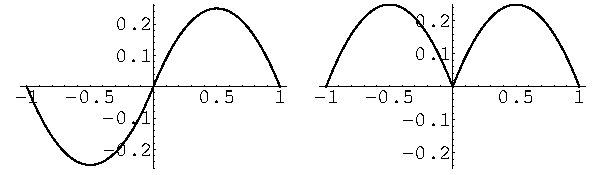
\includegraphics[width=0.6\textwidth]{ode/fourier_series/oddeven}
      \end{center}
      \caption{The odd and even periodic extension.}
      \label{oddeven}
    \end{figure}
    %%
    %%
  \item
    \begin{enumerate}
      %%
    \item
      We substitute $x = 0$ into the cosine series.
      \begin{gather*}
        0 = \frac{1}{6} - \frac{1}{\pi^2} \sum_{n = 1}^\infty \frac{1}{n^2} \\
        \boxed{
          \sum_{n = 1}^\infty \frac{1}{n^2} = \frac{\pi^2}{6}
          }
      \end{gather*}
      %%
    \item
      We substitute $x = 1/2$ into the cosine series.
      \begin{gather*}
        \frac{1}{4} 
        = \frac{1}{6} - \frac{1}{\pi^2} \sum_{n = 1}^\infty \frac{\cos(n \pi)}{n^2} \\
        \boxed{
          \sum_{n = 1}^\infty \frac{(-1)^n}{n^2} = - \frac{\pi^2}{12}
          }
      \end{gather*}
      %%
    \item
      We substitute $x = 1/2$ into the sine series.
      \begin{gather*}
        \frac{1}{4} = \frac{8}{\pi^3} \sum_{n = 1}^\infty \frac{\sin((2n-1) \pi/2 )}{(2n-1)^3} \\
        \boxed{
          \sum_{n = 1}^\infty \frac{(-1)^n}{(2n-1)^3} = - \frac{\pi^3}{32}
          }
      \end{gather*}
    \end{enumerate}
  \end{enumerate}
\end{Solution}







\raggedbottom
}
